% !TEX root = main.tex
\chapter{実験結果}
本章では3.1節ではブロードコンタクトレーザー、3.2節ではリッジ導波路型レーザーへの電流注入実験についての結果を報告する。
\section{ブロードコンタクトレーザー試料に関する測定結果}%=====================================
ブロードコンタクトレーザーへ定常電流を流してILカーブ\adsppp{(注入電流vs発光強度の曲線)}を得る実験を行った。様々な共振器長$L$、電極パッド幅$w$の試料に対して実験を行うことで閾値電流$I_{th}$などのウエハの基本的な物性パラメータを見積もることが目的である。

具体的には発振閾値電流$I_{\rm{th}}$を測定することに加えて、発振時の印可電流の増分に対する光出力の増大から発光量子効率(外部量子効率$\eta_{d}$)を見積もる。外部量子効率の逆数と共振器長の関係から内部量子効率$\eta_{int}$および内部損失$\alpha_{int}$を得る。さらに発振閾値電流から閾値電流密度$J_{th}$を算出し共振器長の逆数との関係から透明電流密度$J_{0}$と微分モード利得$\Gamma g_{0}$を得る。

%また発振閾値電流密度を算出するためにデバイス内の電流の広がりを見積もった。
3周期歪量子井戸ブロードコンタクトレーザーと10周期歪補償量子井戸ブロードコンタクトレーザーで節を分けた。
\subsection{3周期歪量子井戸ブロードコンタクトレーザー}%===============================
3周期歪量子井戸ブロードコンタクトレーザーの結果を示す。図\ref{fig:fig_3_1_3QW_broacdcontact_IL}(a)縦軸を発光強度(片方の端面)、横軸を電流としたILカーブの結果を示す。また図\ref{fig:fig_3_1_3QW_broacdcontact_IL}(b)は縦軸を試料にかかっている電圧、横軸を電流としたIVカーブの結果である。共振器長$L$が$L$=500、 1000、 2000\si{ \micro\metre}の結果をプロットした。代表としてパッド幅$w$=50\si{ \micro\metre}の結果をプロットした。印可電流は1\si{ \micro\metre}パルスを2 ms繰り返し周期で流しており、デューティー比は1:2000である。

\begin{figure}[h]
	\centering
	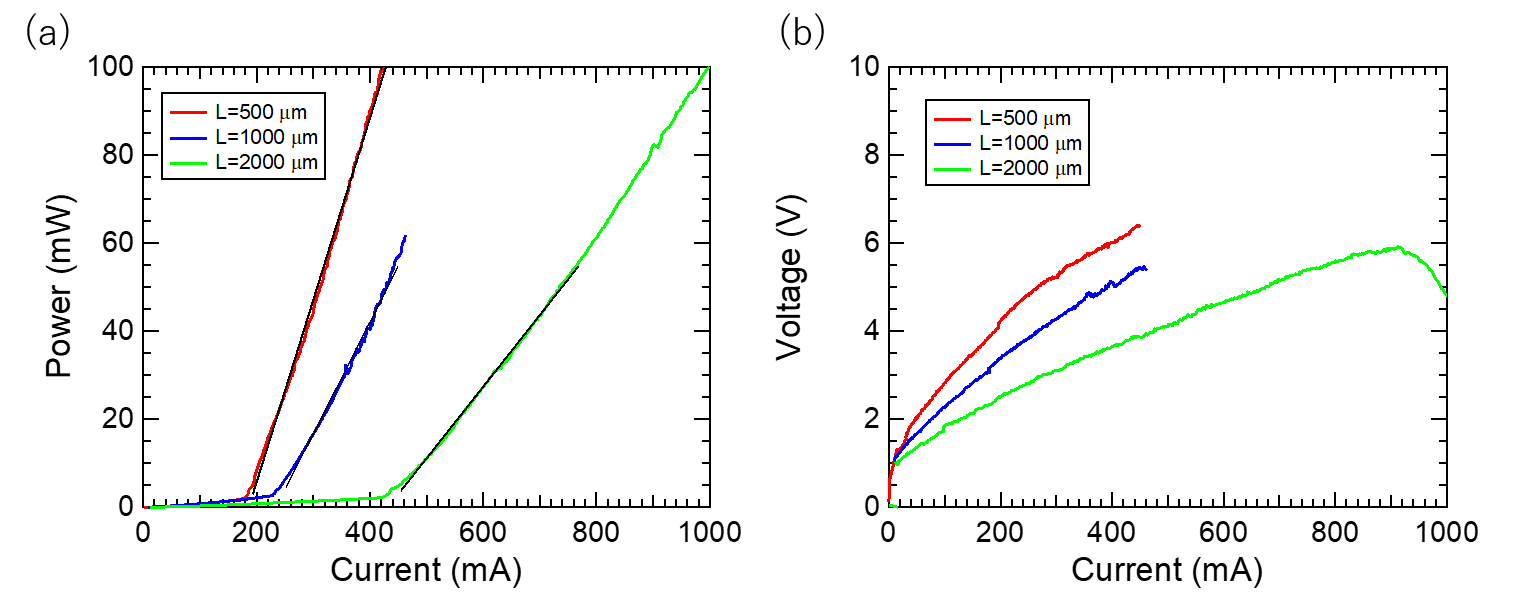
\includegraphics[width=15cm]{figure/fig_3_1_3QW_broadcontact_IL.png}
		\caption{3周期歪量子井戸ブロードコンタクトレーザーのILカーブ(a)およびIVカーブ(b)}
		\label{fig:fig_3_1_3QW_broacdcontact_IL}
\end{figure}

図\ref{fig:fig_3_1_3QW_broacdcontact_IL}(a)を見ると各デバイスにおいて電流値を上げてくと光出力強度が増加していき、ある電流値を超えると発振が始まり発光強度が急激に増加することがわかる。その閾値電流値を発振しているときのILカーブを直線フィッティングすることで求めた。フィッティング直線の$x$切片を発振閾値電流$I_{\rm{th}}$とした。またフィッティング直線の傾きから発振時のスロープ効率2$\Delta P/\Delta I$を得た。スロープ効率はフィッティングの傾きにデューティー比を乗じ(DC電流注入での発光量に換算するためにデューティ比が1:1000であれば1000倍する)、さらに共振器の両端面からの放出を考慮して2倍にして算出した。
図\ref{fig:fig_3_1_3QW_broacdcontact_IL}(a)のILカーブの値を表\ref{table:table_3_1_3QW_broadcontact}に示す。
\begin{table}[h]
  \caption{3周期ブロードコンタクトレーザーの閾値電流}
  \label{table:table_3_1_3QW_broadcontact}
  \centering
  \begin{tabular}{ccc}
    \hline
    共振器長$L$\ ($\si{\micro\metre}$)  & 閾値電流$I_{th}$ (mA)  & Slope 2$\Delta P/\Delta I$ (W/A) \\
    \hline \hline
     500& 187&  0.83  \\
    1000& 234& 0.51\\
    2000& 450&0.37\\
       \hline
  \end{tabular}
\end{table}



図\ref{fig:fig_3_1_3QW_broacdcontact_IL}(b)を見ると各デバイスにおいて電流が流れ始めるのが1 V付近からでありダイオード特性が見られる。また共振器長$L$が長いほど同じ電流に対する電圧が低い。これは共振器長$L$に比例して電流が流れる面積が大きくなるためデバイスの抵抗値が小さくなっているためである。


次に様々なパッド幅に対して見積もった発振閾値電流$I_{\rm{th}}$の結果を図\ref{fig:fig_3_1_3QW_broadcontact_Ith}(a)に示す。発振閾値電流$I_{\rm{th}}$、横軸が電極パッド幅$w$である。図\ref{fig:fig_3_1_3QW_broadcontact_Ith}(b)は発振時の発光効率は$2 \Delta P/\Delta I$である。

図\ref{fig:fig_3_1_3QW_broadcontact_Ith}(a)を見ると、パッド幅$w$が50\si{ \micro\metre}より大きい領域では閾値電流$I_{\rm{th}}$はパッド幅$w$に対して線形に増加した。一方パッド幅$w$が小さい領域では線形に変化していない。

この原因は電流がパッド幅$w$に対して無視できないほど広がってしまっているためだと考えられる。電流広がりについてはフィッティングから見積もった。詳しくは3.1.3節で述べる。

図\ref{fig:fig_3_1_3QW_broadcontact_Ith}(b)を見るとそれぞれの共振器長でパッド幅$w$が大きいところでは概ね横ばいの値を持っている。2$\Delta P/\Delta I$はパッド幅$w$に依存しないことがわかる。幅$w$は光の増幅を受ける方向とは関係がなく直感と一致する。

\begin{figure}[h]

	\centering
	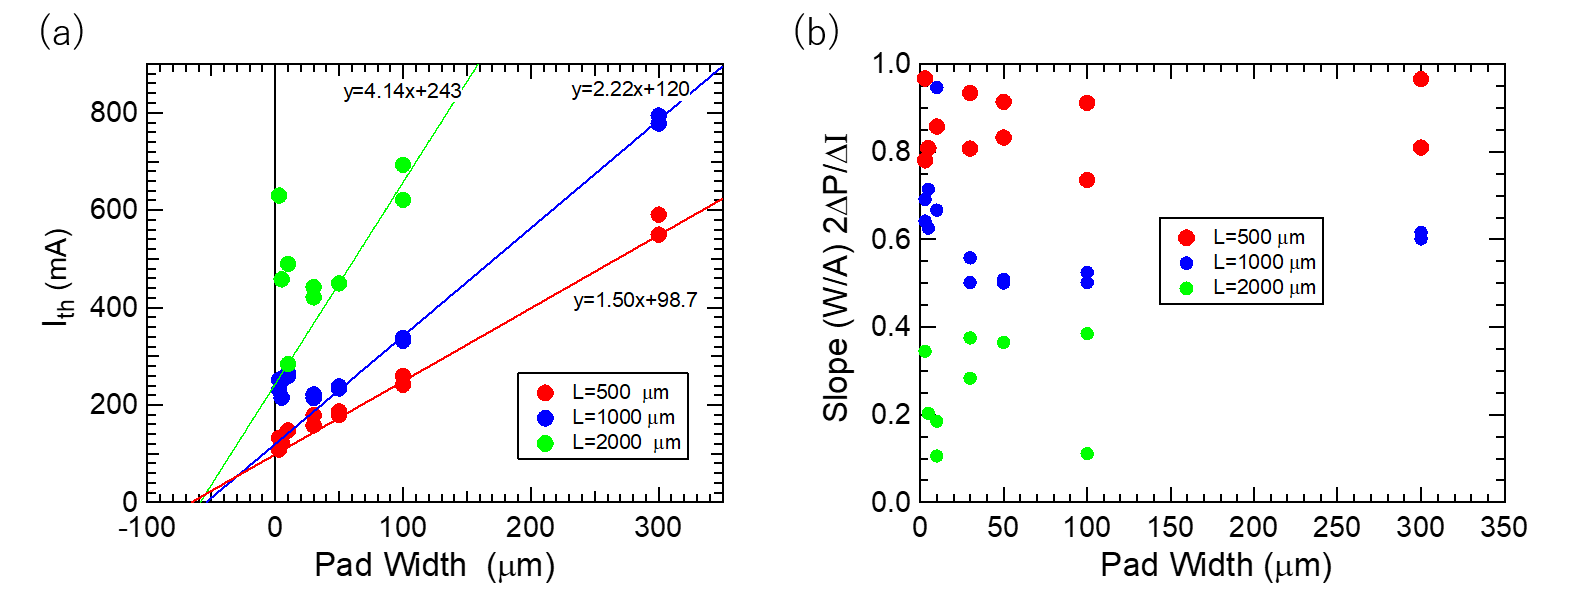
\includegraphics[width=15cm]{figure/fig_3_1_3QW_broadcontact_Ith.png}
	\centering
		\caption
		%[3周期歪量子井戸ブロードコンタクトレーザーの閾値電流とスロープ効率]
		{3周期歪量子井戸ブロードコンタクトレーザーの閾値電流とパッド幅の関係(a)及びスロープ効率とパッド幅の関係(b)}
		%\protect\linebreak (a)閾値電流とパッド幅の関係、(b)スロープ効率とパッド幅の関係 }
		\centering
		\label{fig:fig_3_1_3QW_broadcontact_Ith}
\end{figure}
\clearpage
\subsection{10周期歪補償量子井戸ブロードコンタクトレーザー}%===============================
次に10周期歪補償量子井戸ブロードコンタクトレーザーについての結果を示す。図\ref{fig:fig_3_1_10QW_broadcontact_IL}(a)にILカーブ、(b)にIVカーブを示す。パッド幅$w$=50 \si{\micro\metre}を例としてプロットした。
%色分けは共振器長の違いを表す。
電流は2 \si{\micro s}パルスを2 ms繰り返し周期で印可した。デューティー比は1:1000である。
\begin{figure}[h]
	\centering
	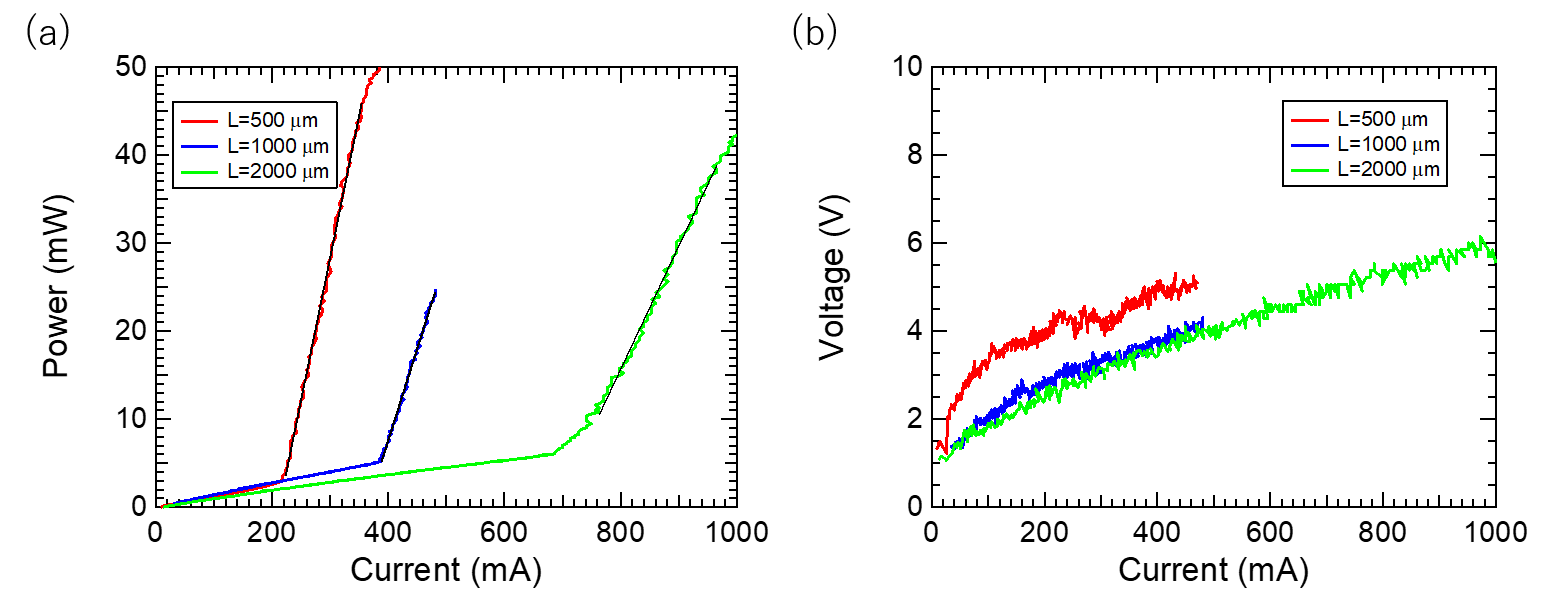
\includegraphics[width=15cm]{figure/fig_3_1_10QW_broadcontact_IL.png}
		\caption{10周期歪補償量子井戸ブロードコンタクトレーザーのILカーブ(a)及びIVカーブ(b)}
		\label{fig:fig_3_1_10QW_broadcontact_IL}
\end{figure}

%典型的な値として図
図\ref{fig:fig_3_1_10QW_broadcontact_IL}(a)のILカーブフィッティング結果の値を表\ref{table:table_3_1_10QW_broadcontact}に示す。傾きはデューティー比1:1000と両端面からの発光を換算していることに注意されたい。
\begin{table}[h]
  \caption{10周期歪補償ブロードコンタクトレーザーの閾値電流}
  \label{table:table_3_1_10QW_broadcontact}
  \centering
  \begin{tabular}{ccc}
    \hline
    共振器長$L$\ (\si{\micro\metre})  & 閾値電流$I_{th}$ (mA)  & Slope 2$\Delta P/\Delta I$ (W/A) \\
    \hline \hline
     500& 212&  0.64  \\
    1000& 363& 0.42\\
    2000& 501&0.27\\
       \hline
  \end{tabular}
\end{table}

次に\adsp02{図}\ref{fig:fig_3_1_3QW_broadcontact_Ith} (a)に\ref{fig:fig_3_1_10QW_broadcontact_IL} (a)のILカーブの発振時の直線フィッティング結果から求めた閾値電流$I_{\rm{th}}$および(b)スロープ効率2 $\Delta P/\Delta I$をパッド幅$w$に対してプロットした。
\begin{figure}[h]
	\centering
	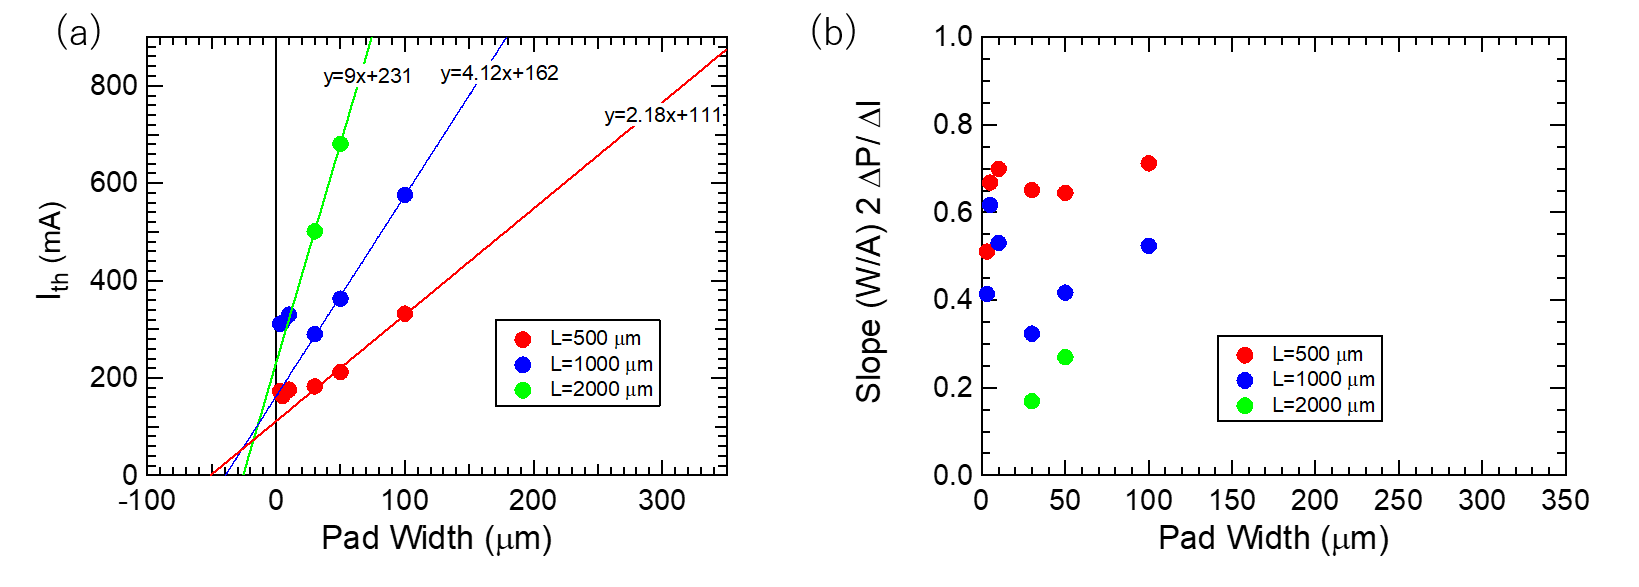
\includegraphics[width=15cm]{figure/fig_3_1_10QW_broadcontact_Ith.png}
		\caption{10周期歪補償量子井戸ブロードコンタクトレーザーの閾値電流とパッド幅の関係(b)及びスロープ効率とパッド幅の関係(b)}
		\label{fig:fig_3_1_10QW_broadcontact_Ith}
\end{figure}
\subsection{電流広がり評価に用いたモデル}%==================
%このことは考えず、このことは考えるそういうモデルのもとで広がりはこのように評価される。
本項では図\ref{fig:fig_3_1_3QW_broadcontact_Ith}(a)や図\ref{fig:fig_3_1_10QW_broadcontact_Ith}(a)の閾値電流$I_{th}$とパッド幅$w$の関係から閾値電流密度$J_{th}$を見積もるときに用いるモデルについて述べる。
%電流広がり評価に用いたモデルおよび解析結果について述べる。

フィッティングを行うモデルとして以下の2つのモデルが考えうる。
\begin{itemize}
\item 電流一定広がりモデル  

%ある面積$w\times L$を流れる電流の大きさは領域内の平均電流密度$J$を用いて$I=JwL$と書けるが、
電流が活性層付近では本来電流の流れる幅を規定する幅$w$に対して一定の幅$w'$だけ広がっているとして$I_{th}$と$w$の間に
\begin{eqnarray}
I_{\rm{th}}=J_{\rm{th}}(w+w')L
\label{eq:denryu_hirogari}
\end{eqnarray}
という関係が成り立つと仮定するモデル。
%パッド幅の増分$(w+w')$及び閾値電流密度$J_{\rm{th}}$を見積もった。


幅$w$距離$d$の平板コンデンサにおいて$w$が$d$よりも十分に大きい場合には平板の端での電場の広がりが$w$によらず一定であるとみなせるようなポテンシャル問題に類似したモデルである。今考えている試料構造は、電極幅が$w=3\sim 300\ \si{\micro\metre}$、電極から活性層までの距離は$d\simeq 2\ \si{\micro\metre}$である。
\item 2乗平均モデル

閾値電流$I_{th}$とパッド幅$w$の関係を
\begin{eqnarray}
I_{\rm{th}}&=&\sqrt{(J_{\rm{th}}wL)^2+\sigma^2}\\
&=&\sqrt{(J_{\rm{th}}wL)^2+(J_{\rm{th}}w'L)^2}
\label{eq:w_prime}
\end{eqnarray}
という式で表すモデル。$w$が大きい領域では$I=JwL$に従い、$w$が小さい領域では$\sigma$分だけずれるというモデルである。
%分光器のスリット幅$w$に対して分解能が従うようなモデルである。
式(\ref{eq:w_prime})では$\sigma$を$J_{\rm{th}}w'L$としている。拡散の幅$w$と$w'$をもつ2つのガウス関数の畳み込みを行った関数の幅を与えるような形式である。
\end{itemize}
図\ref{fig:fig_3_1_w_prime_figure}にキャリア広がりのイメージ図を示す。
\begin{figure}[h]
	\centering
	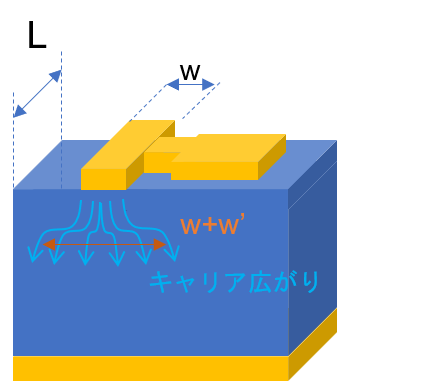
\includegraphics[width=8cm]{figure/fig_3_1_w_prime_figure.png}
	\caption{キャリア広がりのイメージ図}
	\label{fig:fig_3_1_w_prime_figure}
\end{figure}



これらのモデルを用いたフィッティング結果を図\ref{fig:fig_3_1_w_prime}示す。(a)に3周期歪量子井戸レーザーの結果、(b)に10周期歪補償量子井戸レーザーの結果を示す。横軸がパッド幅$w$、縦軸が閾値電流$I_{th}$である。破線はパッド幅$w$が50\ $\si{\micro\metre}$以上の領域を「電流一定広がりモデル」を用いた式(\ref{eq:denryu_hirogari})でフィッティングを行った直線、実線は「2乗平均モデル」を用いた式(\ref{eq:w_prime})によるフィッティング曲線である。

図\ref{fig:fig_3_1_w_prime}(a)(b)それぞれにおいて「電流一定広がりモデル」フィッティング直線の$x$切片が同程度の値を持っていることから、共振器長によらず一定の電流広がりが起きていると考えられる。次節以降では電流広がり一定として閾値電流密度を見積もった。様々な試料を試作する上ではシンプルなモデルを用いることでより簡便に閾値電流密度を算出し比較できることが大切だと考えたからである。


参考までに表\ref{table:table_w_prime}に「2乗平均モデル」を用いた閾値電流密度の結果を示す。フィッティングの標準偏差1$\sigma$を同時に表記した。「-」はプロットが少なかったために標準偏差を評価できなかったことを意味する。

後述する「電流一定広がりモデル」のフィッティング結果と「2乗平均モデル」の結果を比較すると閾値電流密度、パッド幅の増分と共に類似した値を出していることが確かめられた。

%線形モデルで算出した結果(3周期 : $J_{\rm{th}}=$0.20$\sim$0.35 $\ \si{kA/cm^2}$、10周期 : $J_{\rm{th}}\simeq0.40 \ \si{kA/cm^2}$)と比較すると概ね同じ値を与えることがわかる。

%パッド幅の増分についても比較すると(線形なモデルでは3周期 : $w'=58\sim65\ \si{\micro\metre}$、10周期 : $w'=25\sim51\ \si{\micro\metre}$)オーダーでは変わらないことがわかる。



\begin{figure}[h]
	\centering
	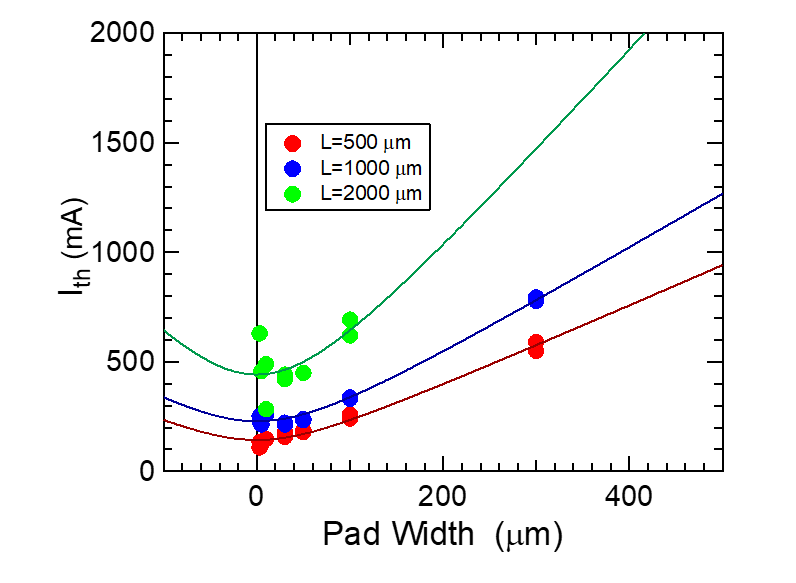
\includegraphics[width=15cm]{figure/fig_3_1_w_prime.png}
	\caption{2つのモデルを用いた閾値電流フィッティング}
	\label{fig:fig_3_1_w_prime}
\end{figure}

\begin{table}[h]
  \caption{2乗平均モデルを用いた閾値電流密度の見積もり結果}
  \label{table:table_w_prime}
  \centering
  \begin{tabular}{cccc}
    \hline
    共振器長$L$ (\si{\micro\metre})  &  閾値電流密度 $J_{\rm{th}} \ (\si{kA/cm^2})$ &$\sigma$\ (\si{mA})& パッド幅の増分  $w'$ (\si{\micro\metre}) \\
    \hline \hline
    3周期歪量子井戸\\
     500 & 0.37 $\pm$ 0.01 & 140 $\pm$ 8&78 $\pm$ 4\\
    1000  & 0.25 $\pm$ 0.01& 230 $ \pm$ 7&92 $\pm$ 3\\
    2000  & 0.23 $\pm$ 0.05& 442 $ \pm$ 42 &96 $\pm$ 24\\
    10周期歪補償量子井戸\\ 
      500 & 0.56 $\pm$ 0.02& 167 $\pm$ 3 &59 $\pm$ 2\\
    1000  & 0.48 $\pm$ 0.04& 300 $\pm$ 14 &63 $\pm$ 6\\
    2000  & 0.58 $\pm$ - & 362 $\pm$ - &31 $\pm$ -\\ 
    \hline
  \end{tabular}
\end{table}
%\begin{comment}

\subsection{電流広がりに関する考察}%==================
3.1.1節と3.1.2節でILカーブから3周期歪量子井戸ブロードコンタクトレーザーと10周期歪補償ブロードコンタクトレーザーについて閾値電流$I_{\rm{th}}$を見積もった。本節では3.1.節で述べた「電流一定広がりモデル」に基づく解析を行い閾値電流密度$J_{th}$を算出した。


%閾値電流密度$J_{\rm{th}}$は半導体レーザーの性能を表す指標にもなるパラメータである。
%レーザーの基本的な特性を知る上で閾値電流密度が大切なパラメータであるからである。発振閾値電流$I_{\rm{th}}$を電流が流れた面積で割ることで閾値電流密度$J_{\rm{th}}$が求まる。

%通常閾値電流$I_{\rm{th}}$は電流を流す面積に比例して大きくなる。面積とは電極パッド幅$w$と共振器長$L$の積で表される。つまり$I_{\rm{th}}$は$w$に対して線形に増加するはずである。しかし図\ref{fig:fig_3_1_3QW_broacdcontact_IL} (a)や\ref{fig:fig_3_1_10QW_broadcontact_IL}(a) を見るとそうなっていない。そこで発振閾値電流$I_{\rm{th}}$が線形に増加する領域を直線フィッティングし、その直線の$x$切片を含めたパッド幅を有効的なパッド幅と考えて閾値電流密度を算出した。まずは有効パッド幅を見積もった。フィッティング関数の$x$切片の絶対値が実質的なパッド幅の増分$w'$である。
3周期歪量子井戸試料と10周期歪補償量子井戸試料の電流広がり幅$w'$の値を表\ref{table:table_3QW_broadcontact_w_eff}と表\ref{table:table_10QW_broadcontact_w_eff}にそれぞれ示した。
\begin{table}[h]
  \caption{3周期歪量子井戸ブロードコンタクトレーザーの電流広がり}
  \label{table:table_3QW_broadcontact_w_eff}
  \centering
  \begin{tabular}{cc}
    \hline
    共振器長$L$ (\si{\micro\metre})  & パッド幅の増分(電流の広がり) $w'$ (\si{\micro\metre})   \\
    \hline \hline
     500 & 65.8  \\
    1000  & 54.1 \\
    2000  & 58.7 \\ 
    \hline
  \end{tabular}
\end{table}

\begin{table}[h]
  \caption{10周期歪補償量子井戸ブロードコンタクトレーザーの電流広がり}
  \label{table:table_10QW_broadcontact_w_eff}
  \centering
  \begin{tabular}{cc}
    \hline
    共振器長$L$ (\si{\micro\metre})  & パッド幅の増分(電流の広がり) $w'$ (\si{\micro\metre})   \\
    \hline \hline
     500 & 51.1  \\
    1000  & 39.5 \\
    2000  & 25.7 \\ 
    \hline
  \end{tabular}
\end{table}

3周期歪量子井戸レーザーでは58 \si{\micro\metre}から65 \si{\micro\metre}程度の広がりであることが見積もられた。10周期歪補償量子井戸レーザーでは25\ \si{ \micro\metre}から51\si{ \micro\metre}の広がりであった。10周期歪補償値量子井戸レーザーでは値のばらつきが大きく$L=500 \ \si{\micro\metre}$の$w'$と$L=2000 \ \si{\micro\metre}$の$w'$を比較すると2倍程度異なってしまっている。これは共振器長$L=2000\ \si{\micro\metre}$の試料について実験結果が少ないため、不確かさが大きくなってしまったためであると考えられる。発振しにくい$L=2000 \ \si{\micro\metre}$の試料に対しては大電流を流して発振させ、プロットを増やすことが必要である。


この表の値$w'$と閾値電流$I_{\rm{th}}$(mA)から式(\ref{eq:Jth})の関係を用いて閾値電流密度$J_{\rm{th}} \rm{(kA/cm^2)}$を算出した。
\begin{eqnarray}
J_{\rm{th}}=\dfrac{I_{\rm{th}}}{(w+w')L}
\label{eq:Jth}
\end{eqnarray}

その結果を示す。図\ref{fig:fig_3_1_3QW_broadcontact_Jth}に3周期歪量子井戸ブロードコンタクトレーザーの閾値電流密度、図\ref{fig:fig_3_1_10QW_broadcontact_Jth}に10周期歪補償量子井戸ブロードコンタクトレーザーの閾値電流密度をプロットした。

\begin{figure}[h]
	\centering
	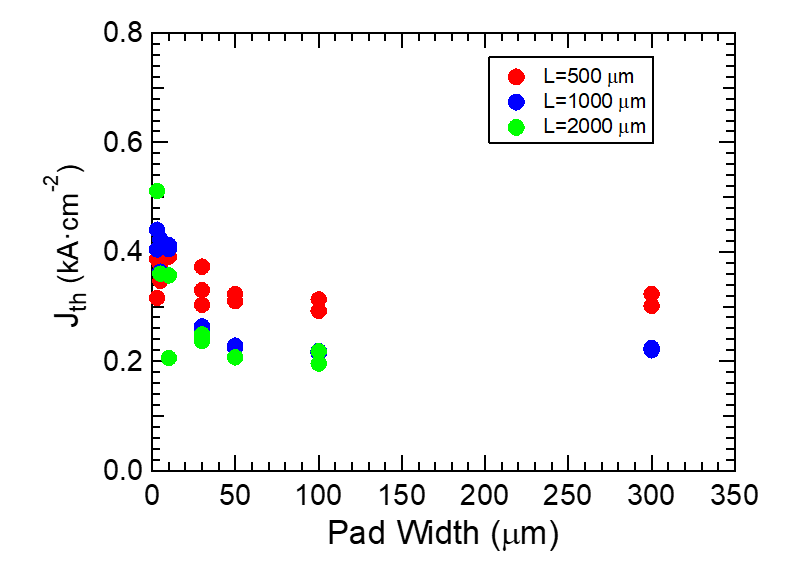
\includegraphics[width=9cm]{figure/fig_3_1_3QW_broadcontact_Jth.png}
		\caption{3周期歪量子井戸ブロードコンタクトレーザーの閾値電流密度}
		\label{fig:fig_3_1_3QW_broadcontact_Jth}
\end{figure}

\begin{figure}[ht]
	\centering
	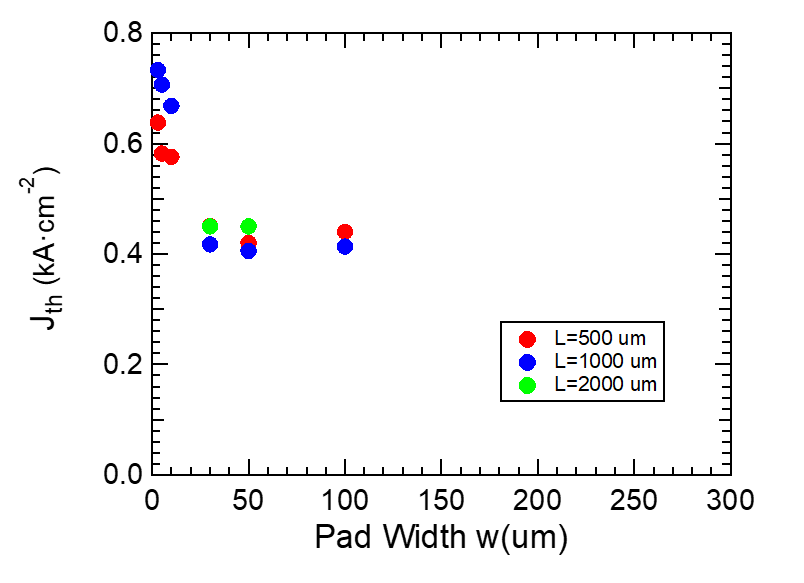
\includegraphics[width=9cm]{figure/fig_3_1_10QW_broadcontact_Jth.png}
		\caption{10周期歪補償量子井戸ブロードコンタクトレーザの閾値電流密度}
		\label{fig:fig_3_1_10QW_broadcontact_Jth}
\end{figure}
閾値電流密度が概ね一定となる$w$が50 \si{\micro\metre}以上の領域で3周期歪量子井戸ブロードコンタクトレーザーでは$0.20\sim 0.35\ \si{ \rm{  kA/cm^{2}}}$、10周期歪補償ブロードコンタクトレーザーでは$0.40\ \rm{  kA/cm^{2}}$程度と見積もられた。

3周期歪量子井戸ブロードコンタクトレーザーでは$w$が50 \si{\micro\metre}より大きい領域で、共振器長が長くなるほど閾値電流密度$J_{\rm{th}}$が小さくなることがわかる。
%これは共振器長が長くなるほどミラーロスに対する内部ロスが大きくなっていき、発振が起こりにくくなっているためである。

一方10周期歪補償量子井戸ブロードコンタクトレーザーでは$L=2000 \si{\micro\metre}$の値が他の2つに比べて大きくなってしまっている。これは$w'$が小さく見積もられており、$J_{\rm{th}}$が大きく見積もられたためだと考えられる。$w'$の解析に用いたプロット点数が少ないことが原因である。

%パッド幅$w$の広がり$w'$が数十\si{\micro\metre}とパッド幅に対して優位なほど広がっているという推察を得たが、この原因としてウエハの結晶構造が考えられる。図\ref{fig:fig_2_1_wafer_structure}のエピウエハ構造において活性層の上のSCH層の上に100 nm厚のp-$\rm{In_{0.485}Ga_{0.515}P}$層が挿入されている。このp-$\rm{In_{0.485}Ga_{0.515}P}$のバンドギャップは1.891 eVは上下を挟んでいるGaAsのバンドギャップ1.424 eVに比べて0.467 eV大きい。このバンドギャップの差によりキャリアが拡散され結晶面内へ広がってしまったと考えられる。
\clearpage
\clearpage
\begin{comment}
\subsection{外部量子効率、内部量子効率と内部損失の計算}%=============
次にILカーブの発振時の傾きに相当するスロープ効率$\Delta P/\Delta I$から試料の内部微分量子効率$\eta_{i}$および内部損失$\alpha$を算出した。まずはスロープ効率$2 \Delta P/\Delta I \rm{ (W/A)}$から外部微分量子効率$\eta_{\rm{d}}$を算出した。式({\ref{eq:eta_d})の関係を用いた。
\begin{eqnarray}
\eta_{\rm{d}}=\dfrac{e}{h\nu}2\dfrac{\Delta P}{\Delta I} 
\label{eq:eta_d}
\end{eqnarray}
eは電気素量、hはプランク定数、$\nu$は発振周波数であり、1050 nmとした。$\eta_{\rm{d}}$はキャリアの注入数に対する取り出せる光子の数の割合である。結果を図\ref{fig:fig_3_1_3QW_broadcontact_id}に示す。縦軸を$\eta_{\rm{d}}$横軸をパッド幅$w$としてプロットした。色分けが共振器長の違いを表している。$L$=500 \si{\micro\metre}では0.7程度、$L$=1000         \si{\micro\metre}では0.4程度、L=400 \si{\micro\metre}では0.3程度の値を持っている。
\begin{figure}[h]
	\centering
	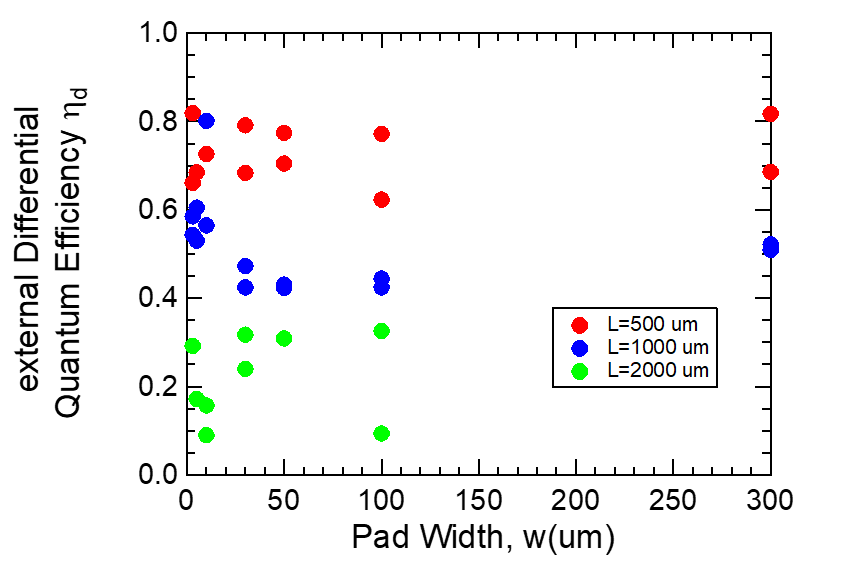
\includegraphics[width=10cm]{figure/fig_3_1_3QW_broadcontact_id.png}
	\caption{3周期歪量子井戸ブロードコンタクトレーザーの外部量子効率}
	\label{fig:fig_3_1_3QW_broadcontact_id}
\end{figure}

ここで$\eta_{d}$は共振器内での全発光にしめる共振器損失の割合であるから
\begin{eqnarray}
\eta_{d}=\eta_{int}\dfrac{\alpha_{m}}{\alpha_{int} +\alpha_{m}}
\end{eqnarray}
である。$\alpha_{int}$は共振器内の平均の内部損失、Rは共振器の端面での反射率、$\eta_{\rm{int}}$は内部微分量子効率である。
$\eta_{\rm{d}}$は共振器長$L$を用いて式(\ref{eq:eta_inverse})と書き表される。
\begin{eqnarray}
\dfrac{1}{\eta_{\rm{d}}}=\dfrac{\alpha_{\rm{int}}}{\rm{ln}(1/R)\eta_{int}}L+\dfrac{1}{\eta_{\rm{int}}}
\label{eq:eta_inverse}
\end{eqnarray}



RはGaAsの屈折率と空気の屈折率の差から0.32と仮定した。見積もった$\eta_{\rm{d}}$の逆数を共振器長に対してプロットし直線フィッティングを行なった。これを図\ref{fig:fig_3_1_3QW_broadcontact_id_inverse}に示す。横軸は共振器長$L$、縦軸に外部微分量子効率の逆数$1/\eta_{\rm{d}}$である。例としてパッド幅$w$=100 \si{\micro\metre}の結果を示す。式(\ref{eq:eta_inverse})よりこのフィッティング直線のy切片から内部量子効率$\eta_{\rm{int}}$を見積もると$\eta_{\rm{int}}$=0.96と計算できる。また、直線の傾きから内部損失$\alpha_{\rm{int}}$を見積もると$\alpha_{\rm{int}}$=11.8 /cmと計算できた。
\begin{figure}[h]
	\centering
	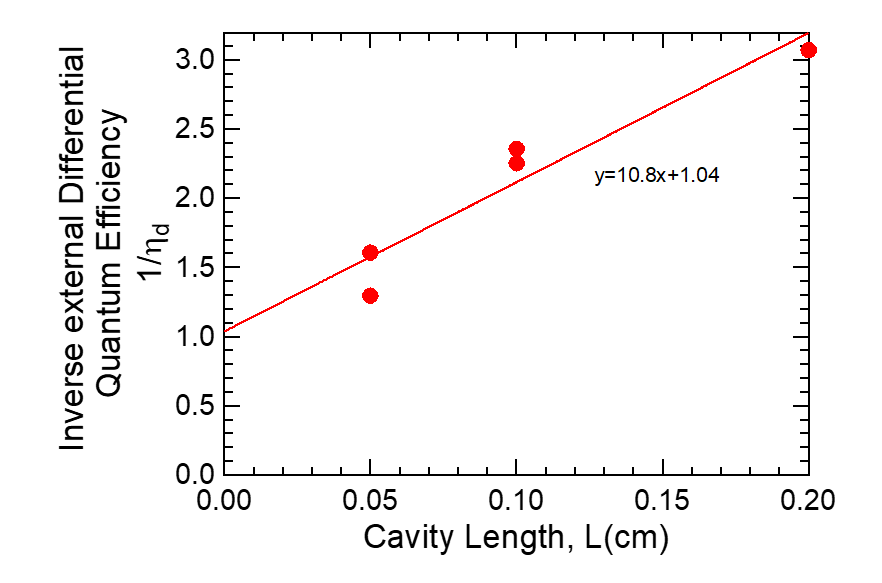
\includegraphics[width=10cm]{figure/fig_3_1_3QW_broadcontact_id_inverse.png}
	\caption{3周期歪量子井戸レーザーの外部量子効率の逆数}
	\label{fig:fig_3_1_3QW_broadcontact_id_inverse}
\end{figure}



\newpage

同様の解析を10周期歪補償量子井戸ブロードコンタクトレーザーの結果についても行った。図\ref{fig:fig_3_1_10QW_broadcontact_id}に外部微分量子効率、図\ref{fig:fig_3_1_10QW_broadcontact_id_inverse}\adsp02{に外部微分量子効率の逆数の共振器長依存性を示す。横軸は共振器長$L$、縦軸は外部微分量子効率の逆数$1/\eta_{\rm{d}}$である。}$w$=50\si{ \micro\metre} の結果を示している。10周期に関しては$\eta_{\rm{int}}$=0.94、$\alpha_{\rm{int}}$=18.0 (/cm)となった。
\begin{figure}[h]
	\centering
	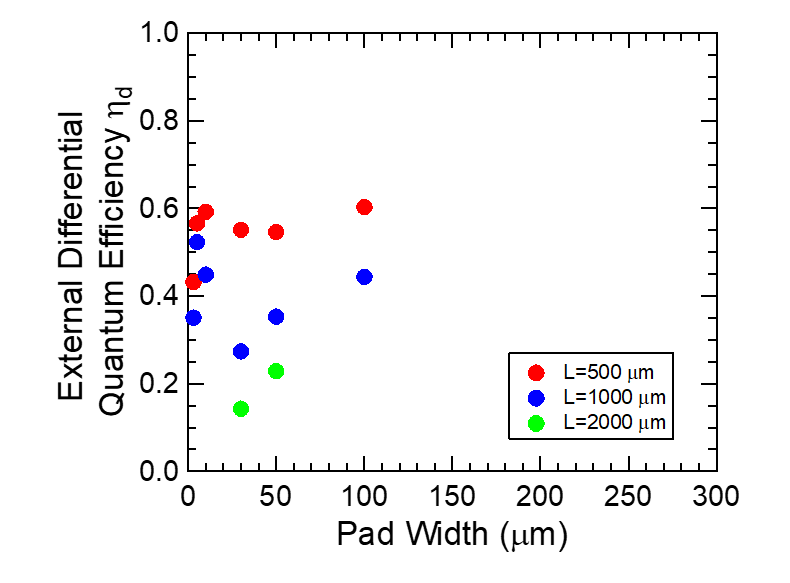
\includegraphics[width=10cm]{figure/fig_3_1_10QW_broadcontact_id.png}
	\caption{10周期歪補償量子井戸レーザーの外部量子効率}
	\label{fig:fig_3_1_10QW_broadcontact_id}
\end{figure}

\begin{figure}[h]
	\centering
	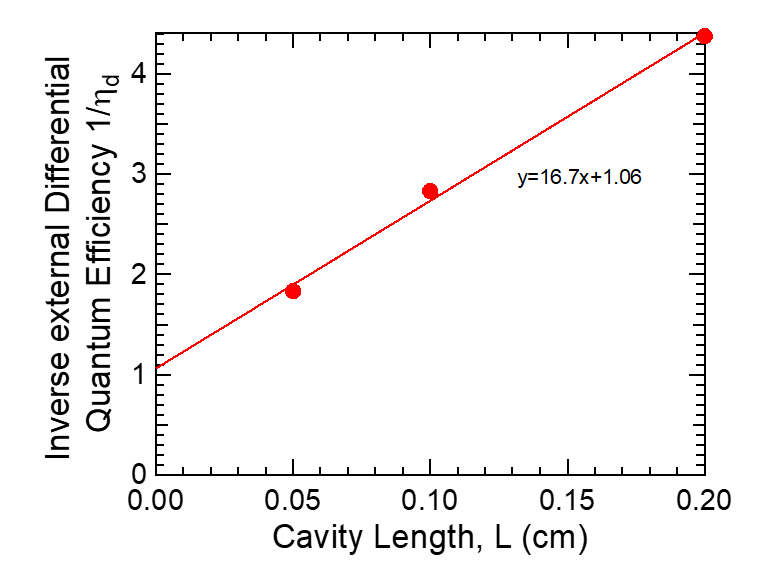
\includegraphics[width=10cm]{figure/fig_3_1_10QW_broadcontact_id_inverse.png}
	\caption{10周期歪補償量子井戸レーザーの外部量子効率の逆数}
	\label{fig:fig_3_1_10QW_broadcontact_id_inverse}
\end{figure}
\end{comment}
\clearpage
\subsection{外部量子効率、内部量子効率と内部損失の計算}%=============
ILカーブの発振時の傾きに相当するスロープ効率$\Delta P/\Delta I$から試料の外部量子効率$\eta_{d}$、内部量子効率$\eta_{i}$および内部損失$\alpha$を算出した。外部量子効率$\eta_{d}(無次元)$は注入したキャリアの増分と共振器から取り出された光子数の増分の比を表す。内部量子効率$\eta_{i}$(無次元)は注入したキャリアのうち、発光再結合しかつ導波路モードに結合したキャリアの割合を表す。内部損失$\alpha_{int}\ (\si{/cm})$は導波路内部での光の吸収や散乱による減衰の大きさを表す係数である。(光強度は光が導波路内部を$x\si{(cm)}$進むうちに$\exp(-\alpha_{int} x)$倍となる)

まずは発振時のスロープ効率$2 \Delta P/\Delta I \rm{ (W/A)}$は式({\ref{eq:eta_d})の関係を用いて外部量子効率$\eta_{\rm{d}}$へと換算できる。
\begin{eqnarray}
\eta_{\rm{d}}=\dfrac{e}{h\nu}2\dfrac{\Delta P}{\Delta I} 
\label{eq:eta_d}
\end{eqnarray}
$e$は電気素量、$h$はプランク定数、$\nu$はレーザーの発振波長であり、解析においては1050 nmとした。
%外部量子効率$\eta_{\rm{d}}$はキャリアの注入数に対する取り出せる光子の数の割合である。


さらに$\eta_{d}$は導波路モードに結合した光の損失のうち、ミラー損失により共振器外部に取り出された光の割合であるから内部量子効率$\eta_{i}$を用いて
\begin{eqnarray}
\eta_{d}=\eta_{int}\dfrac{\alpha_{m}}{\alpha_{int} +\alpha_{m}}
\label{eq:i_d}
\end{eqnarray}
と書ける。$\alpha_{int}$は共振器内の平均の内部損失、$\alpha_{m}$はミラー損失である。ミラー損失$\alpha_{m}$は共振器長$L$と端面の反射率$R$を用いて$\alpha_{m}=1/L\ln (1/R)$と書ける。これを用いて式(\ref{eq:i_d})を変形すると以下のように表すことができる。
%$\eta_{\rm{d}}$は共振器長$L$を用いて式(\ref{eq:eta_inverse})と書き表される。
\begin{eqnarray}
\dfrac{1}{\eta_{\rm{d}}}=\dfrac{\alpha_{\rm{int}}}{\rm{ln}(1/R)\eta_{int}}L+\dfrac{1}{\eta_{\rm{int}}}
\label{eq:eta_inverse}
\end{eqnarray}



解析において反射率$R$はGaAsの屈折率と空気の屈折率から0.32と仮定した。

%以下見積もった$\eta_{\rm{d}}$の逆数を共振器長に対してプロットし直線フィッティングを行った。
\subsubsection{3周期歪量子井戸レーザーの外部量子効率、内部量子効率及び内部損失の計算}
図\ref{fig:fig_3_1_3QW_broadcontact_id_02}に3周期歪量子井戸レーザーの外部量子効率と共振器長の関係を示す。横軸か共振器長$L\ (\si{\micro\metre})$、縦軸が外部量子効率$\eta_{d}$である。共振器長$L$が長いほど外部量子効率$\eta_{d}$が小さくなることがわかる。

\begin{figure}[h]
	\centering
	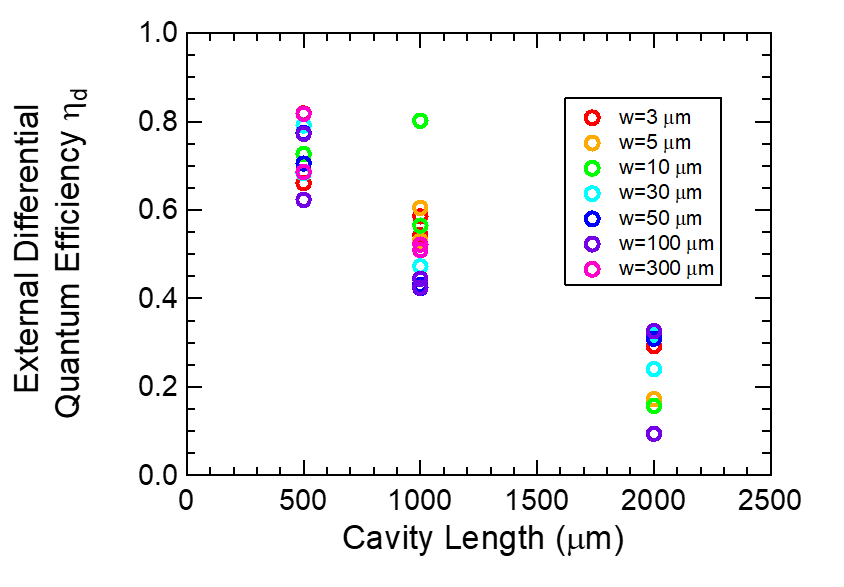
\includegraphics[width=9cm]{figure/fig_3_1_3QW_broadcontact_id_02.png}
	\caption{3周期歪量子井戸レーザーの外部量子効率と共振器長の関係}
	\label{fig:fig_3_1_3QW_broadcontact_id_02}
\end{figure}

図\ref{fig:fig_3_1_3QW_broadcontact_id_inverse_02}に3周期歪量子井戸レーザーの外部量子効率の逆数と共振器長の関係を示す。横軸が共振器長$L\ (\si{cm})$、縦軸が外部量子効率の逆数$1/\eta_{d}$である。内部損失の単位を$\si{(/cm)}$として算出するために共振器長の単位を($\si{cm}$)とした。また、まずは図\ref{fig:fig_3_1_3QW_broadcontact_id_inverse_02}の全てのデータが同じ重みであると扱って、全てのパッド幅$w$に対して同様に行ったフィッティング直線を示す。 


%色分けは同様にパッド幅$w$の違いを表す。

\begin{figure}[h]
	\centering
	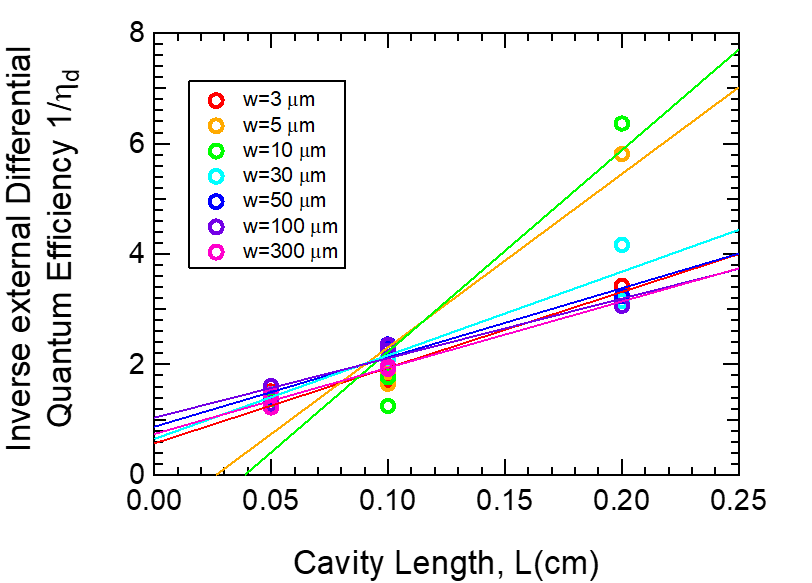
\includegraphics[width=9cm]{figure/fig_3_1_3QW_broadcontact_id_inverse_02.png}
	\caption{3周期歪量子井戸レーザーの外部量子効率の逆数と共振器長の関係}
	\label{fig:fig_3_1_3QW_broadcontact_id_inverse_02}
\end{figure}
図\ref{fig:fig_3_1_3QW_broadcontact_id_inverse_02}の直線フィッティングの結果を表\ref{table:table_3QW_i_d_fit}にまとめる。フィッティングの標準偏差1$\sigma$を同時に表記した。「-」はプロットが少なかったために標準偏差を評価できなかったことを意味する。

表\ref{table:table_3QW_i_d_fit}のフィッティング結果から式(\ref{eq:eta_inverse})の関係を用いて算出した内部量子効率$\eta_{i}$と内部損失$\alpha_{int}$の計算結果を表\ref{table:table_3QW_i_int}にまとめる。標準偏差はばらつきが正規分布に従うとした場合の誤差伝搬の関係を用いて算出した。

あとで述べる外れた点を含まないパッド幅に対してフィッティングを行った結果を各表に追加で示す。($w=50\sim300\ \si{\micro\metre}$をまとめて解析した。)

図\ref{fig:fig_3_1_3QW_broadcontact_id_inverse_02}を見ると共振器長が長くなるほど外部量子効率の逆数1/$\eta_{d}$が線形に増大する系統的な振る舞いが見られる。しかし$L=0.1\ \si{cm}$での$w=10\ \si{\micro\metre}$のプロット(緑)、$L=0.2\ \si{cm}$での$w=5, \ 10,\  30\ \si{\micro\metre}$のプロット(黄色、緑、水色)が外れている。

パッド幅$w$が小さい試料に関してはフォトリソグラフィプロセスの難しさなどの要因により不確かさが大きくなってしまったと考えられる。

\begin{table}[h]
  \caption{3周期歪量子井戸レーザーの外部量子効率逆数のフィッティング結果}
  \label{table:table_3QW_i_d_fit}
  \centering
  \begin{tabular}{ccc}
    \hline
    パッド幅$w$ (\si{\micro\metre})  &  内部量子効率の逆数 $1/\eta_{\rm{int}} $ & $\alpha/(\ln(1/R)\eta_{\rm{int}})\ $ \\
    \hline \hline
     3 & 0.570 $\pm$ 0.204  & 13.71 $\pm$ 1.79 \\
    5  & -0.829 $\pm$\ -\ & 31.39 $\pm$\ -\\
    10  & -1.412 $\pm$\ -\  & 36.45 $\pm$\ -\\ 
    30& 0.654 $\pm$ 0.330& 15.12 $\pm$ 2.49\\
    50& 0.873 $\pm$ 0.218&12.53 $\pm$ 1.91 \\
    100& 1.0367 $\pm$ 0.223& 10.78 $\pm$ 1.95\\
    300&0.742 $\pm$ 0.189 & 11.98 $\pm$ 2.39\\
    \hline
    50 $\sim$ 300 & 0.862 $\pm$ 0.0.114 & 12.07 $\pm$ 1.08\\
    \hline

  \end{tabular}
\end{table}


%式(\ref{eq:eta_inverse})の関係を用いて算出した内部量子効率$\eta_{i}$および内部損失$\alpha$の結果を表\ref{table:table_3QW_i_int}にまとめる。
\begin{table}[h]
  \caption{3周期試料のパッド幅ごとの内部量子効率及び内部損失}
  \label{table:table_3QW_i_int}
  \centering
  \begin{tabular}{ccc}
    \hline
    パッド幅$w$ (\si{\micro\metre})  &  内部量子効率 $\eta_{\rm{int}} $ &内部損失 $\alpha\ $\ (/\si{cm}) \\
    \hline \hline
     3 & 1.75 $\pm$ 0.63 & 27.4 $\pm$ 10.4  \\
    5  & -1.21 $\pm$\ - & -43.1 $\pm$\ -\\
    10  & -0.71 $\pm$\ - & -29.4 $\pm$\ -\\ 
    30& 1.53 $\pm$ 0.77& 26.3 $\pm$ 14.0\\
    50& 1.15 $\pm$ 0.29&16.4 $\pm$ 4.8 \\
    100& 0.96 $\pm$ 0.21& 11.8 $\pm$ 3.3\\
    300&1.35 $\pm$ 0.34 & 18.4 $\pm$ 6.0\\
    \hline
    50$\sim$300& 1.15 $\pm$ 0.15 & 15.9 $\pm$ 2.5\\
    \hline
  \end{tabular}
\end{table}


表\ref{table:table_3QW_i_int}を見ると$w=3\ \si{\micro\metre}$においては内部量子効率$\eta_{\rm{int}}$が標準偏差1$\sigma$の範囲を超えて1より大きくなっている。また$w=5, 10\ \si{\micro\metre}$において内部量子効率$\eta_{\rm{int}}$が負の値を持っている。$w=30\  \si{\micro\metre}$では不確かさが大きくなってしまっている。
そこで全てのプロットを同じ重みで扱うのではなく、パッド幅$w$が大きい試料をまとめて議論するのが適切であると考えた。

より系統的なデータが得られていると考えられる$w=50,\ 100,\ 300\ \si{\micro\metre}$のプロットについて行ったフィッティングの結果を表の最下段に示す。
この結果では内部量子効率は標準偏差2$\sigma$の範囲ないで1程度の高い値をとった。
%これらについて以下のような考察を行った。


%\cdot スロープ効率2$\Delta P/Delta I$算出のためのILカーブフィッティングの際に発振直後をフィットしたため、誘導放出の効果が支配的ではない領域の効率を見積もってしまった。このため、スロープ効率2$\Delta P/Delta I$および外部量子効率$\eta_{d}$が低く見積もられてしまった。そのために$1/\eta_{d}$が高くなってしまった。
\begin{comment}
\begin{itemize}
%\item レーザーデバイスの品質のばらつきが大きい
\item 内部量子効率が負となる要因

プロットの算出方法に問題があったためと考えられる($L=0.20\ \si{\micro\metre}$での緑$L=10\ \si{\micro\metre}$、黄色$L=5\ \si{\micro\metre}$プロットが異常に高い値を示している)。外部量子効率$\eta_{d}$はILカーブの発振領域を直線フィットして得られるスロープ効率2$\Delta P/\Delta I$から算出したものであった。外部量子効率$\eta_{d}$が異常な値を持っているプロットに関して、スロープ効率2$\Delta P/\Delta I$算出のためのILカーブフィッティングの際に誘導放出の効果が支配的ではない領域の効率を見積もってしまった。具体的には発振直後のIL領域である。このためスロープ効率2$\Delta P/\Delta I$および外部量子効率$\eta_{d}$が低く見積もられてしまった。これにしたがって$1/\eta_{d}$が異常に高くなってしまったと考えられる。
%(付録にILカーブを載せるのが良いか全部?)

測定において共振器長が大きい試料では発振閾値電流が大きくなるため、十分な発振領域を得るために短共振器と比較して大きな電流が必要となる。測定で用いた駆動系では十分な電流が得られなかったために、「発振は確認できたがスロープ効率を見積もるには不十分」な大きさの電流までのデータしか得られなかった試料があった。このような不十分なデータに対して発振領域のILカーブ直線フィッティングを行ったために低いスロープ効率が算出されてしまったと考えられる。電流源としてより強力なものを用いて測定を行うといった対策が必要である。

\item 内部量子効率が1よりも大きくなる要因


内部量子効率が高く算出された1つの要因として光検出の際にInGaAs活性層からの発光のみならず、p-GaAs 層(p-InGaP層の直上)からの発光も検出してしまったことが考えられる。障壁となるp-InGaP層の上のp-GaAs層にキャリアがたまり発光が起こっていると推測される。ブロードコンタクトレーザーの測定ではフィルタを用いていないため、GaAsの発光も検出してしまった。InGaAs発光波長帯を切り出して測定を行うことが必要である。追加実験として行ったFIB加工試料の測定結果(付録5.2)ではGaAsの発光波長領域をカットするフィルタの有無でILカーブの発光量の差が生じている。

\end{itemize}
\end{comment}
\begin{comment}
図\ref{fig:fig_3_1_3QW_broadcontact_id_inverse_02}で分かるようにこれらのパッド幅では$L=0.2\ \si{cm}$でのプロットが非常に大きくなっていることが原因だと考えられる。これはスロープ効率が低く見積もられたことに起因する。
また表\ref{table:table_3QW_i_int}の$w=3\ \si{\micro\metre}$では内部量子効率$\eta_{\rm{int}}$が1より大きくなってしまっているがILカーブの直線フィット領域が短く、また発振直後であったため正確に発振効率と見積もれていないと考えられる。$w=300\ \si{\micro\metre}$は発振に必要な電流が大きく発振しにくかったため、$L=2000\ \si{\micro\metre}$のプロットが得られなかったことにより標準偏差1$\sigma$の範囲を超えても内部量子効率が1を超えたと考えられる。

$w=30, 50, 100\ \si{\micro\metre}$に関しては標準偏差1$\sigma$の範囲内で内部量子効率が1程度、内部損失が18\ $\si{/cm}$程度となった。
\end{comment}

%これらのデータはフィッティング誤差が大きいため、さらに異なる共振器長の試料を作製しプロットを増やすことによりフィッティング精度の向上が必要と言える。

%以下の3周期歪量子井戸レーザーの解析においては内部損失$\alpha_{int}$が必要となる。例としてもっとも多くの点をフィットした$w=30\sim300\ \si{\micro\metre}$の結果を用いる。

以下の3周期歪量子井戸レーザーの解析において内部損失$\alpha_{int}$が必要となるが、$w=50\sim300$をまとめてフィッティングした結果を用いる。
\clearpage
\subsubsection{10周期歪補償量子井戸レーザーの外部量子効率、内部量子効率及び内部損失
の計算}
10周期歪補償量子井戸レーザーについても同様の解析を行った。

図\ref{fig:fig_3_1_10QW_broadcontact_id_02}に10周期歪量子井戸レーザーの外部量子効率$\eta_{d}$と共振器長$L$の関係を示す。共振器長が長いほど外部量子効率が小さくなることがわかる。

図\ref{fig:fig_3_1_10QW_broadcontact_id_inverse_02}に10周期歪量子井戸レーザーの外部量子効率の逆数と共振器長の関係及びそれらの直線フィットを示す。

表\ref{table:table_10QW_i_d_fit}に図\ref{fig:fig_3_1_10QW_broadcontact_id_inverse_02}でのフィッティング結果を示す。標準偏差1$\sigma$も併記した。「-」はプロットが少なく標準偏差を算出できなかったことを意味する。

表\ref{table:table_10QW_i_d_fit}のフィッティング結果から式(\ref{eq:eta_inverse})の関係を用いて算出した内部量子効率$\eta_{int}$及び内部損失$\alpha_{int}$の結果を表\ref{table:table_10QW_i_int}にまとめる。

\begin{figure}[h]
	\centering
	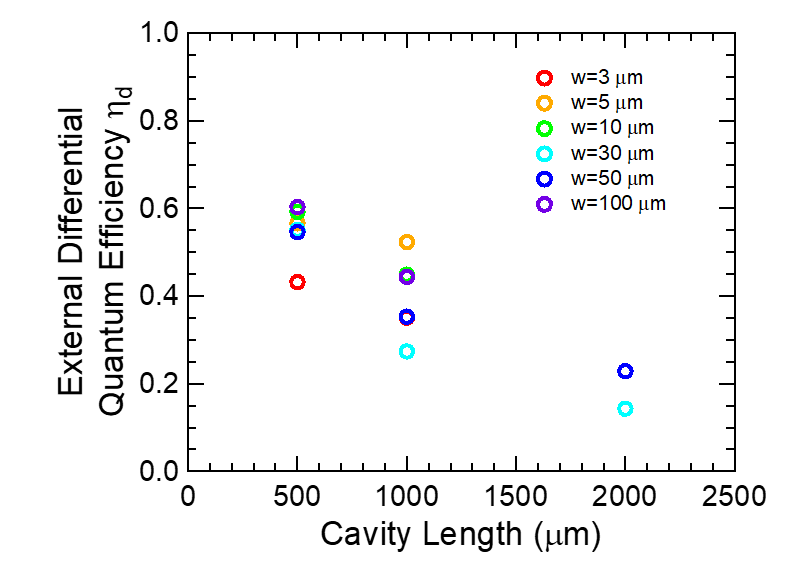
\includegraphics[width=9cm]{figure/fig_3_1_10QW_broadcontact_id_02.png}
	\caption{10周期歪補償量子井戸レーザーの外部量子効率と共振器長の関係}
	\label{fig:fig_3_1_10QW_broadcontact_id_02}
\end{figure}

\begin{figure}[h]
	\centering
	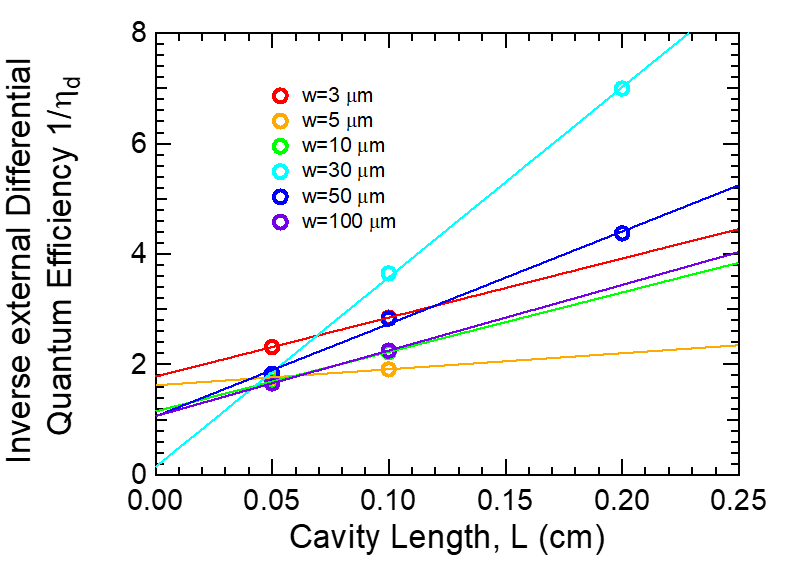
\includegraphics[width=9cm]{figure/fig_3_1_10QW_broadcontact_id_inverse_02.png}
	\caption{10周期歪補償量子井戸レーザーの外部量子効率の逆数と共振器長の関係}
	\label{fig:fig_3_1_10QW_broadcontact_id_inverse_02}
\end{figure}
\begin{table}[h]
  \caption{10周期歪補償量子井戸レーザーの外部量子効率逆数のフィッティング結果}
  \label{table:table_10QW_i_d_fit}
  \centering
  \begin{tabular}{ccc}
    \hline
    パッド幅$w$ (\si{\micro\metre})  &  内部量子効率の逆数 $1/\eta_{\rm{int}} $ & $\alpha/(\ln(1/R)\eta_{\rm{int}})\ $ \\
    \hline \hline
     3 & 1.781 $\pm$ \ -  & 10.684 $\pm$\ - \\
    5  & 1.622 $\pm$\ -\  & 2.905 $\pm$\ -\\
    10  & 1.151 $\pm$\ -\  & 10.76 $\pm$\ -\\ 
    30& 0.143 $\pm$ 0.107& 34.37 $\pm$ 0.81\\
    50& 1.060 $\pm$ 0.149&16.73 $\pm$ 1.13 \\
    100& 1.065 $\pm$\ -& 11.88 $\pm$ -\\
    300&- & -\\
    \hline
    50, 100  &0.840\ $\pm$\ 0.235& 17.48\ $\pm$\ 2.06\\ 
    \hline
  \end{tabular}
\end{table}

\newpage


\begin{table}[h]
  \caption{10周期歪補償量子井戸レーザー内部量子効率及び内部損失}
  \label{table:table_10QW_i_int}
  \centering
  \begin{tabular}{ccc}
    \hline
    パッド幅$w$ (\si{\micro\metre})  &  内部量子効率 $\eta_{\rm{int}} $ &内部損失 $\alpha\ (\si{/cm}) $ \\
    \hline \hline
     3 & 0.56 $\pm$ \ -  & 6.8 $\pm$\ - \\
    5  & 0.62 $\pm$\ -\ &2.0 $\pm$\ -\\
    10  & 0.87 $\pm$\ -\  & 10 $\pm$\ -\\ 
    30& 7.0 $\pm$ 5.2& 2.7$\times 10^2$ $\pm$ 2.0$\times 10^2$\\
    50& 0.94 $\pm$ 0.13&18.0 $\pm$ 2.5 \\%18 $\pm$ 2.5 
    100& 0.94 $\pm$\ -& 13 $\pm$\ -\\
    300&- &-\\
    \hline
    50, 100 &1.18 $\pm$\ 0.33 & 23.7 $\pm$ 7.2\\
    \hline
  \end{tabular}
\end{table}

表\ref{table:table_10QW_i_int}を見ると$w=3, 5, 10 \ \si{\micro\metre}$では内部量子効率$\eta_{int}$は0.56$\sim$0.87の値である。$w=30\ \si{\micro\metre}$では内部量子効率$\eta_{int}$は7.0という値をもつ。$w=50, 100 \ \si{\micro\metre}$では0.94程度の値を持っている。
\begin{comment}
内部量子効率が7.0と異常に高くなってしまった要因について考察した。
\begin{itemize}
\item $w=30\ \si{\micro\metre}$で内部量子効率$\eta_{int}$が7.0という非常に大きい値を与えた原因

この原因は共振器長$L=0.2\ \si{cm}$のプロットが非常に大きくなったためだと考えられる($L=0.2\ \si{cm}$の水色プロット値 : 6.5程度)。このプロットに関しては3周期試料で高い値を与えたプロットと同様に、ILカーブの直線フィッティングの領域が発振閾値に近い領域であったため、スロープ効率が低く見積もられた。
電流を多く流すことができなかった理由の1つとして温度上昇による電極の劣化が見られたことがあげられる(プローバーと電極の接触抵抗によるジュール熱に伴う電極の焦げ)。
\end{itemize}
\end{comment}
$w=30\ \si{\micro\metre}$以外のデータにおいても$L=2000\ \si{\micro\metre}$でのプロットがないなど、プロットが少なく不確かさ評価ができていないという問題がある。より厳密に値を算出するためにはプロットを増やす必要があると言える。

10周期試料の結果についても3周期試料と同様に$w$が大きい試料の結果を重視して解析を行った。$w=50, \ 100\ \si{\micro\metre}$のプロットに重みを置きそれらをフィットすることにより得た結果を各表の下段に示す。

$w=50, \ 100\ \si{\micro\metre}$をまとめて解析した値において内部量子効率$\eta_{int}$は標準偏差$1\sigma$の範囲内で1程度の高い値を持っている。
%\end{comment}


以下の10周期歪補償量子井戸レーザーの解析において$w=50, \ 100\ \si{ \micro\metre}$の結果を例として用いる。

\clearpage
\subsection{透明電流密度の見積もり}

次に透明電流密度$J_{0}$の見積もりを行った。透明電流密度$J_{0}$は3周期試料と10周期試料の井戸数の違いを反映する物理量である。共振器内の正味の利得$g_{\rm{net}}$は
\begin{eqnarray}
g_{\rm{net}}=\Gamma G-\alpha_{int}-\alpha_{m}
\label{eq:eta_j0}
\end{eqnarray}
と書ける。線形利得$G=g_{0}(J-J_{0})$を仮定すると閾値電流密度は
\begin{eqnarray}
J_{th}=J_{0}+\dfrac{\alpha_{int}}{\Gamma g_{0}}+\dfrac{1}{\Gamma g_{0}}\rm{ln}\left(\dfrac{1}{R}\right)\dfrac{1}{L}
\label{eq:j_th}
\end{eqnarray}
と書ける。この式にしたがうと$J_{\rm{th}}$は$1/L$に比例する。図\ref{fig:fig_3_1_3QW_broadcontact_j0}に$1/L$に対して$J_{\rm{th}}$をプロットした。色分けは共振器長を表す。
\begin{figure}[h]
	\centering
	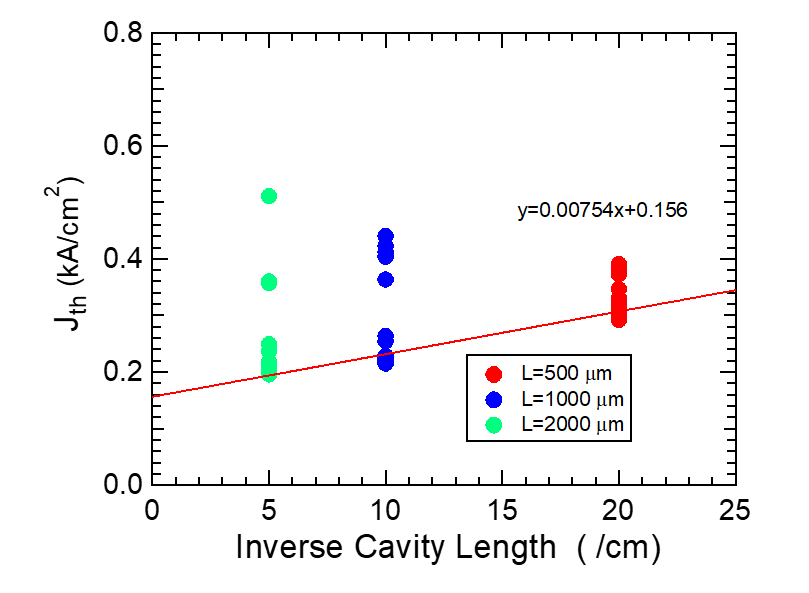
\includegraphics[width=10cm]{figure/fig_3_1_3QW_broadcontact_j0.png}
	\caption{3周期歪量子井戸ブロードコンタクトレーザーの透明電流密度の見積もり}
	\label{fig:fig_3_1_3QW_broadcontact_j0}
\end{figure}

図\ref{fig:fig_3_1_3QW_broadcontact_j0}のプロットのなかで、図\ref{fig:fig_3_1_3QW_broadcontact_Jth}の閾値電流密度をプロットした図において$J_{\rm{th}}$が一定となっている$w$が50 \si{\micro\metre}以上のプロットに対して線形フィッティングを行った。赤い直線がフィッティング直線である。フィッティング結果と式(\ref{eq:j_th})の関係を用いて$\Gamma g_{0}$と$J_{0}$を見積もると$\Gamma g_{0}=151 \ \pm \ 11\ \rm{ cm/kA}$、$J_{0}=0.0782 \ \pm \ 0.0240 \ \rm{kA/cm^{2}}$を得た。%算出には例として$w=100\ \si{\micro\metre}$の結果を用いた。


10周期歪補償量子井戸ブロードコンタクトレーザーについても同様の解析を行った。図\ref{fig:fig_3_1_10QW_broadcontact_j0}に$J_{\rm{th}}$対$1/L$のプロットを示す。フィッティング結果から$\Gamma g_{0}$と$J_{0}$を見積もると$\Gamma g_{0}=558\   \pm \ 292\  \si{cm/kA}$、$J_{0}=0.357\  \pm\  0.024\  \rm{kA/cm^{2}}$を得た。
%算出には例として$w=50\ \si{\micro\metre}$の結果を用いた。
\begin{figure}[t]
	\centering
	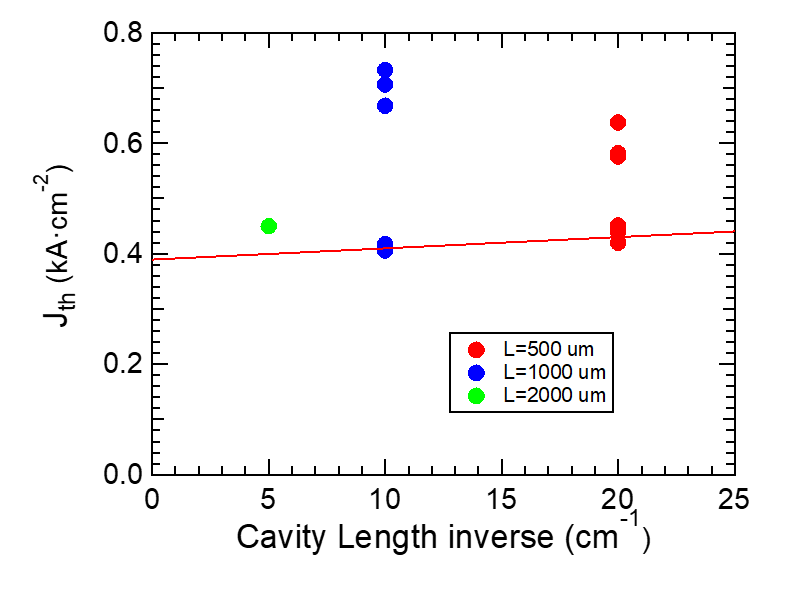
\includegraphics[width=10cm]{figure/fig_3_1_10QW_broadcontact_j0.png}
	\caption{10周期歪補償量子井戸ブロードコンタクトレーザーの透明電流密度の見積もり}
	\label{fig:fig_3_1_10QW_broadcontact_j0}
\end{figure}
\newpage
\subsection{ブロードコンタクトレーザーに対する電流注入実験のまとめと考察}

実験結果をまとめると3周期歪量子井戸ブロードコンタクトレーザーと10周期歪補償ブロードコンタクトレーザーに関して以下の表のようになる。
%\begin{comment}
\begin{table}[h]
  \caption{ブロードコンタクトレーザーの結果まとめ}
  \label{table:table_I0}
  \centering
  \begin{tabular}{lcccc}
    \hline
    試料   &  内部損失$\alpha_{int}\  \rm{ /cm}$&内部量子効率$\eta_{int} $&透明電流密度 $J_{0} \ \rm{  kA/cm^2}$  &$\Gamma g_{0}$ cm/kA\\
    \hline \hline
     3周期 &   15.9 $\pm$ 2.5 &1.15 $\pm$ 0.15&0.051 $\pm$  0.020& 151 $\pm$ 11\\
    10周期 & 23.7 $\pm$\ 7.2&1.18 $\pm$ 0.33&0.35 $\pm$\ 0.03&558 $\pm$ 292\\
    \hline
  \end{tabular}
\end{table}
%\end{comment}
%
\begin{comment}
\begin{table}[h]
  \caption{ブロードコンタクトレーザーの結果まとめ}
  \label{table:table_I0}
  \centering
  \begin{tabular}{lcccc}
    \hline
    試料   &  内部損失$\alpha_{int}\  \rm{ /cm}$&内部量子効率$\eta_{int} $&透明電流密度 $J_{0}\  \rm{  kA/cm^2}$  &$\Gamma g_{0}$ cm/kA\\
    \hline \hline
     3周期 &   20.0 $\pm$ 3.8 &1.30\ $\pm$ 0.22&0.024\ $\pm$  0.028& 151\ $\pm$ 11\\
    10周期 & 23.7$\pm$\ 7.2&1.18\ $\pm$ 0.33&0.36\ $\pm$0.02&558\ $\pm$\ 292\\
    \hline
  \end{tabular}
\end{table}
\end{comment}
%内部損失は10周期試料の方が高くなった。


3周期試料と10周期試料を比較したとき透明電流密度は10周期試料が7倍程度高く標準偏差1$\sigma$の範囲を超えて優位な差を得た。層数を増加させた効果が見られたと言える。
%層数の比(活性層の厚さの比に等しい)が3.3倍であることを考えると式(\ref{eq:Mj0})で予想された透明電流密度の比程度大きくなっている。
また微分\adsp02{モード}利得$\Gamma g_{0}$については10周期の方は3周期に比べて3倍程度大きくなった。
モード利得$\Gamma G=\Gamma g_{0}(J-J_{0})$を図\ref{fig:fig_3_1_broadcontact_modal_gain}にプロットした。

\begin{figure}[t]
	\centering
	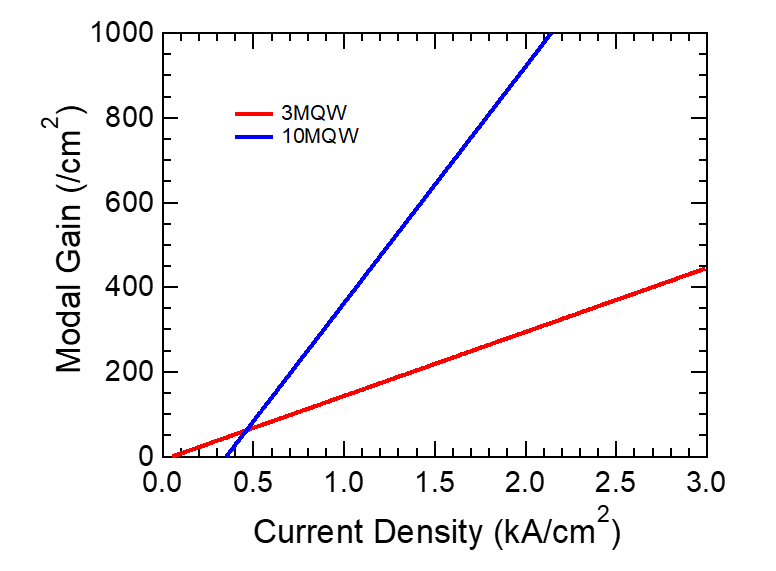
\includegraphics[width=10cm]{figure/fig_3_1_broadcontact_modal_gain.png}
	\caption{モード利得の電流密度依存性の見積もり}
	\label{fig:fig_3_1_broadcontact_modal_gain}
\end{figure}
これを見ると0.5$ \ \rm{kA/cm^2}$ 以下では層数の少ない3周期試料の方がモード利得は大きく、それ以降では10周期試料の方が高いモード利得が得られることがわかる。この振る舞いは図	\ref{fig:fig_gain_mode}の理論計算により求められたモード利得の振る舞いと一致している。
\clearpage
\section{リッジ導波路型レーザーに関する実験結果}%===================
ブロードコンタクトレーザーを用い、半導体レーザーの基本的な特性を調べた。次に完成したデバイスとしてのリッジ導波路型レーザーに短パルス電圧を印可し、利得スイッチング動作を行った。
\subsection{定常電流の結果}

利得スイッチング動作を行う前にまずは発振するか確かめること、および閾値電流を見積もることを目的として定常電流による標準的なデバイス評価実験を行なった。方法はブロードコンタクトレーザーの評価測定と同じである。
\subsubsection{3周期歪量子井戸リッジ導波路型レーザーの結果}
まずは3周期歪量子井戸リッジ導波路型レーザーの結果を示す。2 \si{\micro s}パルスを2 ms周期で印可した。デューティー比は1:1000である。
まずは3周期歪量子井戸リッジ導波路型レーザーの結果を図\ref{fig:fig_3_2_3QW_ridge_IL}に示す。図\ref{fig:fig_3_2_3QW_ridge_IL}(a)はILカーブ、(b)はIVカーブである。色分けは共振器長$L$の違いを表す。

\begin{figure}[h]
	\centering
	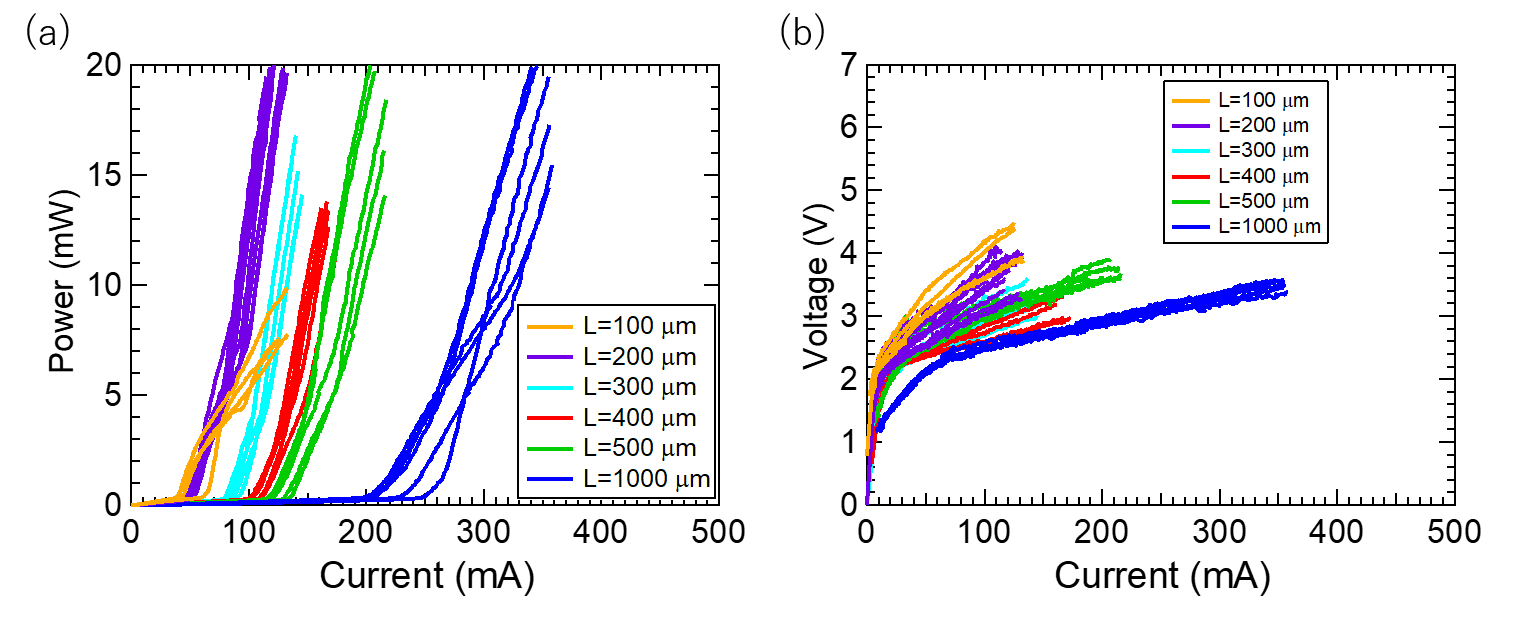
\includegraphics[width=15cm]{figure/fig_3_2_3QW_ridge_IL.png}
		\caption{3周期歪量子井戸リッジ導波路型レーザーのILカーブ(a)およびIVカーブ(b)}
		\label{fig:fig_3_2_3QW_ridge_IL}
\end{figure}


次にILカーブから見積もった閾値電流$I_{\rm{th}}$、$J_{\rm{th}}$と閾値電流密度を図\ref{fig:fig_3_2_3QW_ridge_Ith}に示す。図中の丸プロットが閾値電流$I_{\rm{th}}$であり左の軸に対してのプロットした。十字プロットは閾値電流を共振器長とリッジ幅の積で割った値の閾値電流密度$J_{\rm{th}}$であり右の軸に対してのプロットである。横軸は共振器長である。色分けはリッジ幅の違いを表している。紫色がリッジ幅1.5 \si{\micro\metre}、黄色が2.5 \si{\micro\metre}である。

これを見ると閾値電流は共振器長に対して概ね線形に増加しており\delsp02{最短では}\adsp02{最小の閾値電流は$L$=100 \si{\micro\metre}のときであり}50 mA程度となっている。またリッジ幅を1.5 \si{\micro\metre} 、 2.5 \si{\micro\metre}と変えても閾値電流に差が見られていない。これはブロードコンタクトレーザーで示唆されたように電流が広がってしまい有効的なリッジ幅は実際のリッジ幅よりも広いと考えられる。%したがって閾値電流密度を見積もることは難しい。

閾値電流密度は$L$が300 \si{\micro\metre}より大きい共振器長において概ね横ばいとなっており10から20 $\rm{kA/cm^2}$の値を持っている。またリッジ幅による差異は単に同程度の閾値電流を異なるリッジ幅で割ったためである。


\begin{figure}[h]
	\centering
	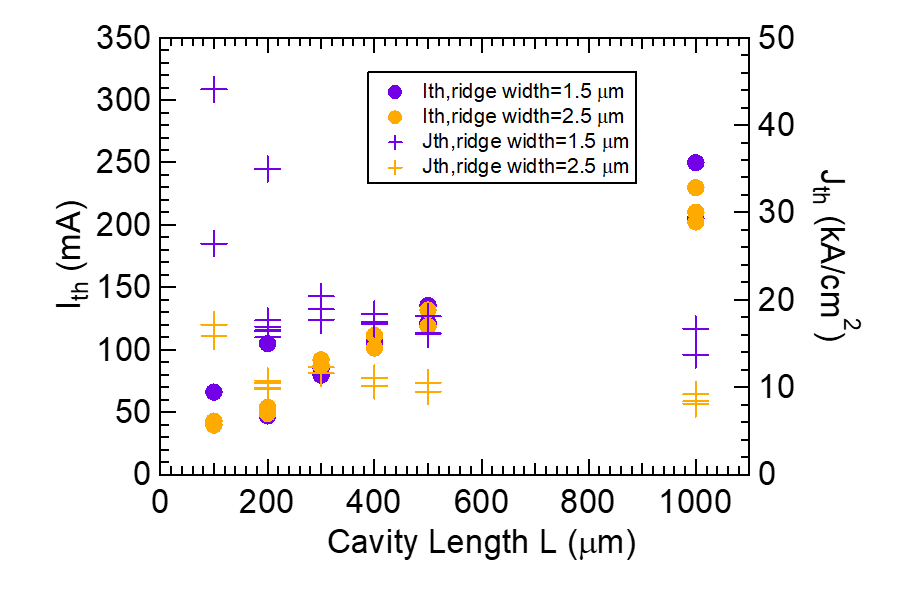
\includegraphics[width=10cm]{figure/fig_3_2_3QW_ridge_Ith.png}
		\caption{3周期歪量子井戸リッジ導波路型レーザーの$I_{\rm{th}}$、$J_{\rm{th}}$}
		\label{fig:fig_3_2_3QW_ridge_Ith}
\end{figure}
次にILカーブの発振領域のスロープ効率$2 \Delta P/\Delta I$および外部量子効率$\eta_{\rm{d}}$を共振器長に対してプロットした結果を図\ref{fig:fig_3_2_3QW_ridge_slope}に示す。全てのプロットが右軸及び左軸に対応し、左軸にスロープ効率$2 \Delta P/\Delta I$、右軸に外部量子効率$\eta_{d}=e/h\nu2\Delta P/\Delta I$を表示した。発光効率$2 \Delta P/\Delta I$は0.03から0.87 W/A の値となった。また外部量子効率は0.026から0.87の値を持っている。
%L=100だけ低くなる原因ある?
\begin{figure}[h]
	\centering
	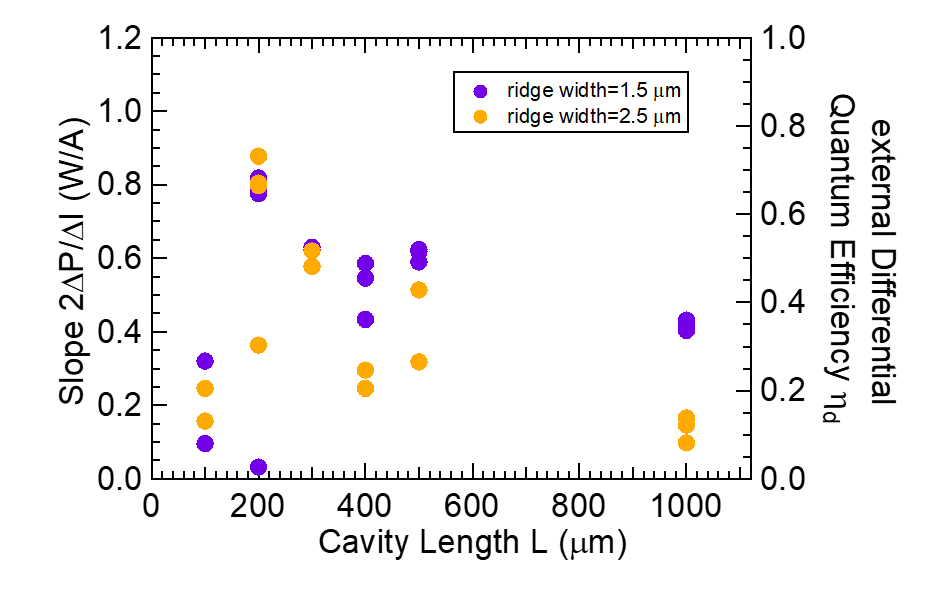
\includegraphics[width=10cm]{figure/fig_3_2_3QW_ridge_slope.png}
		\caption{3周期歪量子井戸リッジ導波路型レーザーのスロープ効率および外部量子効率}
		\label{fig:fig_3_2_3QW_ridge_slope}
\end{figure}

\clearpage
\subsubsection{10周期歪補償量子井戸リッジ導波路レーザー}
次に10周期歪補償量子井戸リッジ導波路レーザーの結果を示す。図\ref{fig:fig_3_2_10QW_ridge_IL}(a)にILカーブ、(b)にIVカーブを示す。

図\ref{fig:fig_3_2_10QW_ridge_IL}(a)を見るとそれぞれの共振器長において発振したことがわかる。$L$= 400\ \si{\micro\metre}の赤い線を見ると$I$= 200 mA付近からどの試料においても発光量が下がってきている(ドループ)。$L$= 300\ \si{\micro\metre}の水色の線においてもまた発光量の下がりが見られる。図\ref{fig:fig_3_2_10QW_ridge_IL}(b)では値の飛びが見られる($L$= 1000\ \si{\micro\metre}、$I$=200 mA付近)。

図\ref{fig:fig_3_2_10QW_ridge_IL}(b)では値の飛びは電圧をモニタしているオシロスコープのレンジ切り替えによる飛びだと考えられる。


\begin{figure}[h]
	\centering
	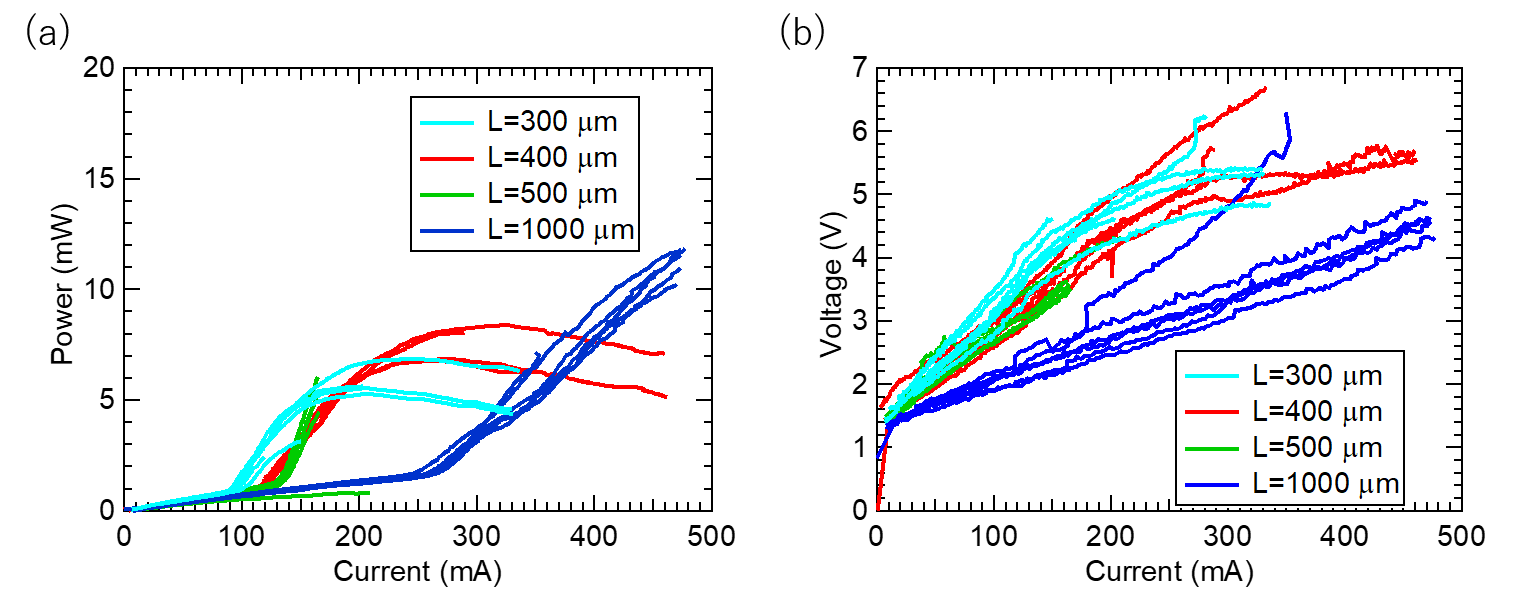
\includegraphics[width=15cm]{figure/fig_3_2_10QW_ridge_IL.png}
		\caption{10周期歪補償量子井戸リッジ導波路型レーザーのILカーブ(a)およびIVカーブ(b)}
		\label{fig:fig_3_2_10QW_ridge_IL}
\end{figure}
次にILカーブから閾値電流$I_{\rm{th}}$と閾値電流密度$J_{\rm{th}}$を算出した。その結果を図\ref{fig:fig_3_2_10QW_ridge_Ith}に示す。閾値電流は共振器長に対して線形に増加しており最小で90 mA程度となった。色分けはリッジ幅の違いを表すが、3周期試料と同様に閾値電流においてリッジ幅による差異は見られない。閾値電流密度は10から20 $\rm{kA/cm^{2}}$程度となったが電流広がりの影響を考えていないため正しく見積もることはできていない。
\begin{figure}[h]
	\centering
	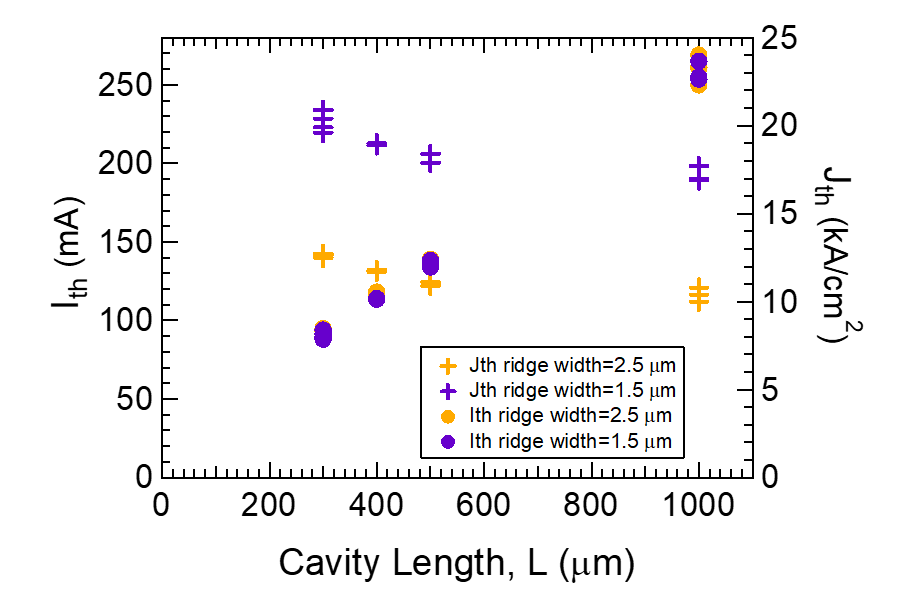
\includegraphics[width=10cm]{figure/fig_3_2_10QW_ridge_Ith.png}
		\caption{10周期歪補償量子井戸リッジ導波路型レーザーの閾値電流と閾値電流密度}
		\label{fig:fig_3_2_10QW_ridge_Ith}
\end{figure}
ILカーブの発振時の傾きから見積もったスロープ効率$2\Delta P/\Delta I$および外部量子効率$\eta_{\rm{d}}$を図\ref{fig:fig_3_2_10QW_ridge_slope}に示す。$\eta_{d}$は発振波長1030 nmとして計算した。

スロープ効率は共振器長$L=300, 400, 1000\ \si{\micro\metre}$では最大でも0.2 W/A程度の値を持っている。$L=500\ \si{\micro\metre}$では他と比べて大きい0.3 W/A程度の値を持っている。

%通常$\eta_{d}$は共振器長に対しては減少するはずであるが(式(\ref{eq:eta_inverse})による)、$L$=300 \si{\micro\metre},  400  \si{\micro\metre}では$L$の増加に対して減少が見られない。図\ref{fig:fig_3_2_10QW_ridge_IL}(a)を見てもこの2種類の共振器長に関してはILカーブが曲がり発光量が減少していることがわかる。



\begin{figure}[ht]
	\centering
	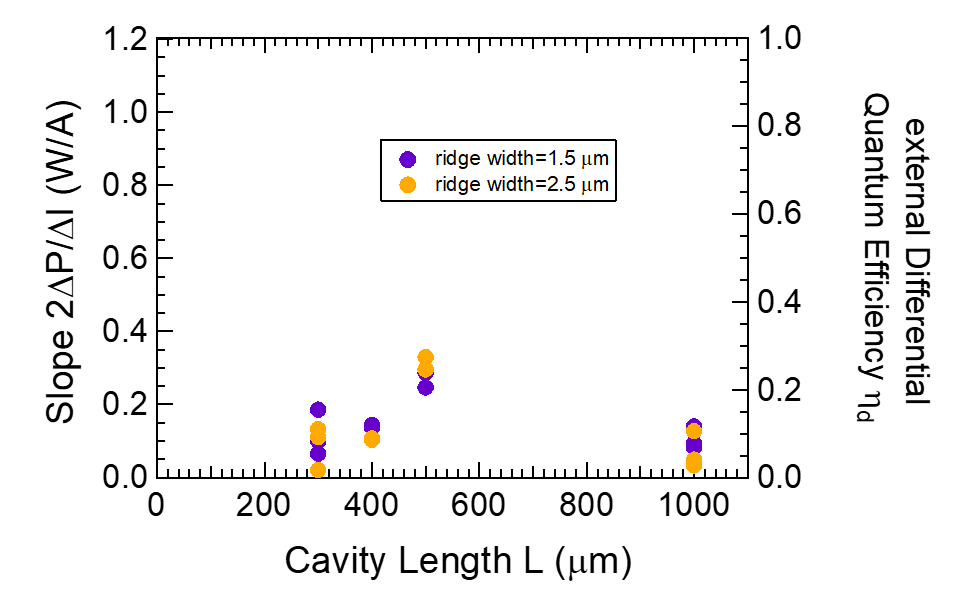
\includegraphics[width=10cm]{figure/fig_3_2_10QW_ridge_slope.png}
		\caption{10周期歪補償量子井戸リッジ導波路型レーザーのスロープおよび外部量子効率}
		\label{fig:fig_3_2_10QW_ridge_slope}
\end{figure}

\subsection{リッジ導波路型レーザーへの定常電流注入実験の結果まとめ}
3周期試料及び10周期試料の両方の試料において発振が確認された。リッジ形成プロセスが問題なく成功したと言える。

%\subsubsection{3周期歪量子井戸試料と10周期歪補償量子井戸試料の比較}
3周期試料と10周期試料を比較すると閾値電流は同程度であり外部量子効率は\delsp02{1}\adsp02{3}周期試料の方が高いという結果を得た。

%また発振する前の発光強度を見てみると10周期試料の方が大きい\delsp02{ことがわかる}。自然放出光の強度が10周期試料の方が大きいことがわかる。
\subsubsection{10周期歪補償リッジ導波路型レーザーのILカーブのドループについて}
ここで10周期歪補償量子井戸リッジ導波路型レーザーのILカーブにおいて観測されたドループ(注入増に対する発光強度減)\delsp02{減衰}について述べる。このような発光量の飽和現象の原因としてはデバイスの温度上昇やそれに伴う内部損失の増大、利得飽和(レート方程式における$\epsilon$の効果)、反射端面の光学損傷、空間のホールバーニング効果などが挙げられる。


本研究では試料の温度上昇に着目しそれを抑制するようなマウントを行ってドループを解消することを試みた。その詳細について付録5.1に記載した。
%これらの中から実験的に原因を特定するためには、発光の遠視野像を撮像することや活性層ではなくp側のGaAs層での発光強度を観察することが良いと考えられる。特に先の実験からInGaP層が障壁の役割をしていると想像されているため、その上下のGaAs層で発光が起こっている可能性が高く、その注入電流に対するGaAs発光強度を測定することができればデバイス内部のキャリアの分布が決められるのではないかと考えられる。
%ここでキャリアの再結合過程を考えると式(\ref{eq:tau_r})の非発光再結合には
%\begin{equation}
%\dfrac{1}{\tau_{nr}}(n)=A_{1}+A_{2}n+A_{3}n^2
%\end{equation}
%とキャリア密度nの二乗に比例するようなオージェ再結合が起こることが知られている。
%ILカーブを見るとこの中で共振器長に対して依存性が
%空間ホールバーニングはモードを確認すれは良い,filamentation(繊維化)

\clearpage
\subsection{ナノ秒パルス電流注入の結果}

次にリッジ導波路型レーザーに関してパルス幅1 ns電気パルスを印可し電流注入利得スイッチング実験を行った。そのILカーブと時間波形を示す。
\subsection{ILカーブ}
短パルス駆動時のILカーブを示す。その際電流に換算することが困難であったため、横軸はパルスの電圧である。
\subsubsection{3周期歪量子井戸レーザーのILカーブ}
図\ref{fig:fig_3_2_3QW_ridge_GS_power}に3周期歪量子井戸リッジ導波路型レーザーのナノ秒パルス駆動時のILカーブを示す。励起パルスのパルス幅は1 nsであり繰り返しは1 MHzである。3つの異なる共振器長において発振が確認できた。共振器長はL=100 \si{\micro\metre}、200 \si{\micro\metre}、300 \si{\micro\metre}である。試料はレーザーバーの状態のものを用いた。\adsp02{1 cm程度芯線をむき出しにした同軸ケーブルを試料から5 mm程度の場所に固定し、芯線とp電極を金線でワイヤリングを行った。作業の都合上$L$=200 \si{\micro\metre}に関してワイヤーの長さは他の試料よりも2 mm程度長くなった。同軸ケーブルのグランド側は試料が乗っている約2 cm角の銅板に密着させた。}\delsp02{むき出しにしたものを試料の近く1cm程度($L$=200 umは3 cm程度と遠い)まで近づけ、芯線とレーザーの電極を金線でワイヤリングを行った。したがって回路全体の特性}インピーダンスマッチング\delsp02{しているか定かでない。}\adsp02{のためのマッチング抵抗の付加などを行っていない。}

\begin{figure}[h]
	\centering
	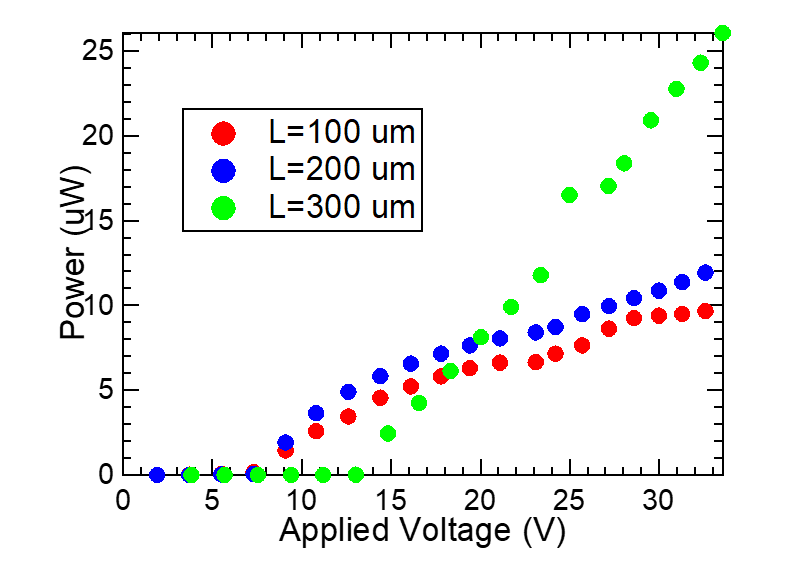
\includegraphics[width=10cm]{figure/fig_3_2_3QW_ridge_GS_power.png}
		\caption{3周期歪量子井戸 短パルス駆動時のILカーブ}
		\label{fig:fig_3_2_3QW_ridge_GS_power}
\end{figure}


\newpage
\subsubsection{10周期歪補償量子井戸レーザーのILカーブ}
次に図\ref{fig:fig_3_2_10QW_ridge_GS_power}に10周期歪補償量子井戸リッジ導波路型レーザーのナノ秒パルス駆動時のILカーブを示す。電気パルスはパルス幅1 ns、繰り返し周期は1 MHzである。共振器長は$L$=300 \si{\micro\metre}、400 \si{\micro\metre}、500 \si{\micro\metre}である。10周期試料は全て\adsp02{1つずつに分離、チップ化しTO-}CANタイプ\adsp02{のキャリアにマウントした}試料である。\delsp02{インピーダンスマッチが取れており、高速電気パルスが形状を崩さず入っているとみなしている。}\adsp02{TO-CANのp側の足をSMAコネクタの芯線とInはんだを用いて導通を取り(距離は0 )、n側の足は5 mm程度の金線空中配線によりSMAコネクタのグランドと繋げた。}インピーダンスマッチのためのマッチング抵抗付加などは行っていない。

図\ref{fig:fig_3_2_10QW_ridge_GS_power}を見ると3つの異なる共振器長の試料に対して発振が確認できた。
%発振閾値書くか?
\begin{figure}[h]
	\centering
	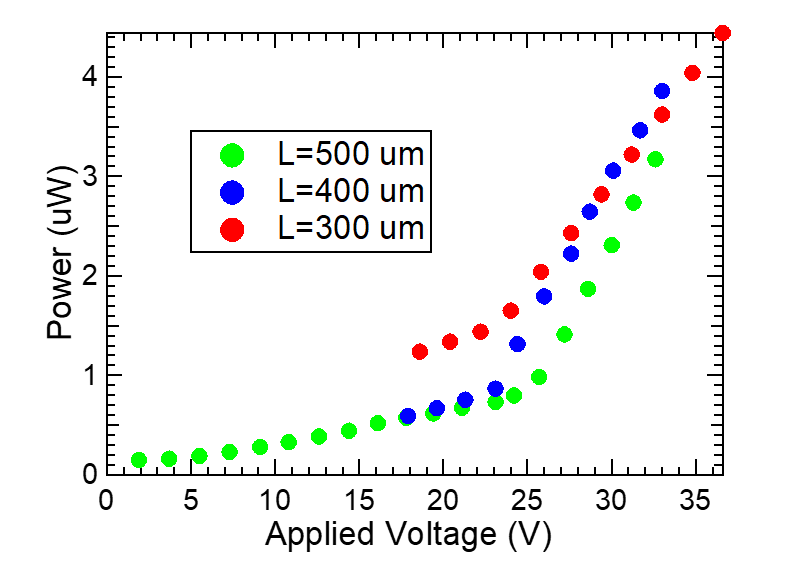
\includegraphics[width=10cm]{figure/fig_3_2_10QW_ridge_GS_power.png}
		\caption{10歪補償量子井戸リッジ導波路型レーザーの短パルス駆動時のILカーブ}
		\label{fig:fig_3_2_10QW_ridge_GS_power}
\end{figure}
\clearpage
\subsection{3周期歪量子井戸試料の利得スイッチング動作}%===============================
次にフォトダイオードで光を検出し高速オシロスコープで電気信号をモニタした時間波形を示す。図\ref{fig:fig_3_2_3QW_ridge_L100_GS}(a)に3周期歪量子井戸レーザーの共振器長$L$=100 \si{\micro\metre}試料の利得スイッチング動作の時間波形を示す。励起強度を変えた実験結果を示す。図\ref{fig:fig_3_2_3QW_ridge_L100_GS}(b)には強度を規格化したプロットをしめす。(a)を見ると励起強度を\delsp02{あげる}\adsp02{増大させる}にしたがってピーク強度が高くなって行くが途中で頭打ちになっている。(b)を見ると21 V程度までは励起強度の増加につれて立ち上がりが早くなっているがそれより強励起ではわずかに遅くなって\delsp02{いって}いる。
\begin{figure}[h]
	\centering
	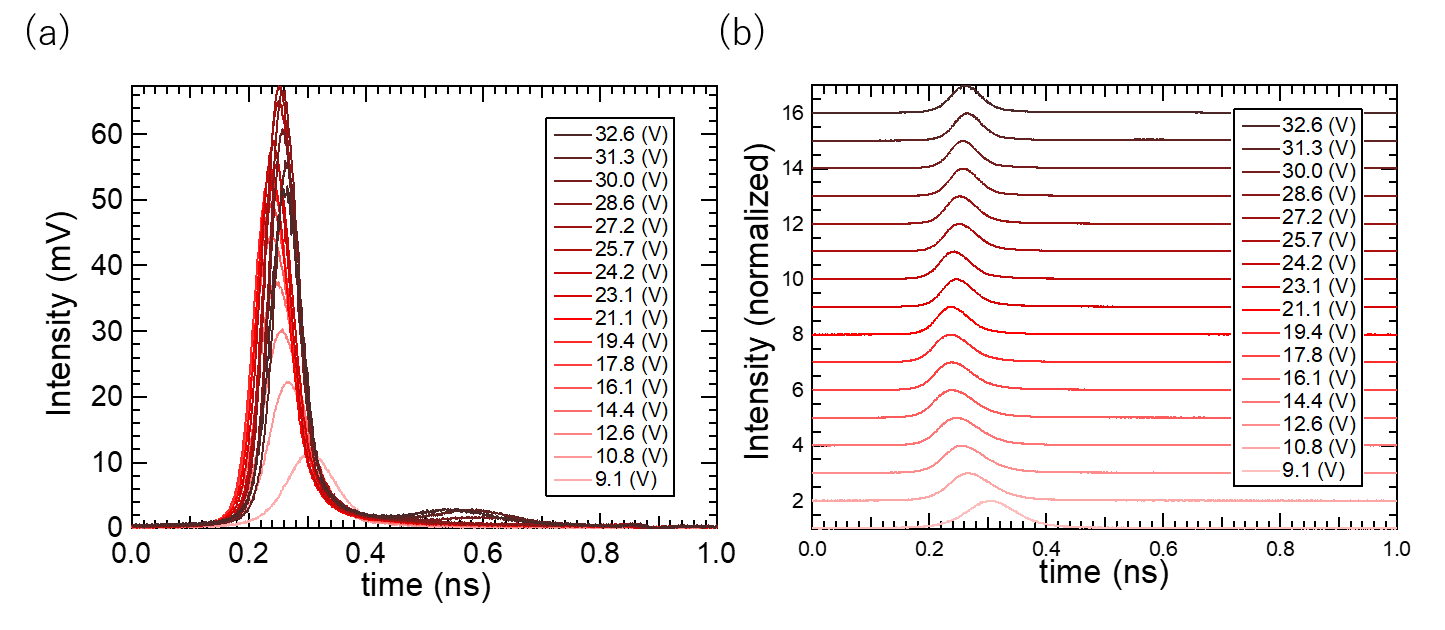
\includegraphics[width=15cm]{figure/fig_3_2_3QW_ridge_L100_GS.png}
		\caption{3周期歪量子井戸レーザー $L$=100 \si{\micro\metre} の利得スイッチング光パルスの時間波形}
		\label{fig:fig_3_2_3QW_ridge_L100_GS}
\end{figure}


図\ref{fig:fig_3_2_3QW_ridge_L200_GS}には$L$=200 \si{\micro\metre}試料の結果を示す。(a)を見ると励起強度を増加させるにしたがって1つめの光パルス強度は途中までは増加するもののあるところから減衰することがわかる。また途中から第2の光パルスが見られる。電流注入利得スイッチングに特有の緩和振動である。(b)を見ると光パルスの立ち上がりは励起強度とともに遅くなっていく様子が見られる。
%2番目のパルスの地上がり時間からなんかわからんの?それが緩和振動なのかどうか


\begin{figure}[h]
	\centering
	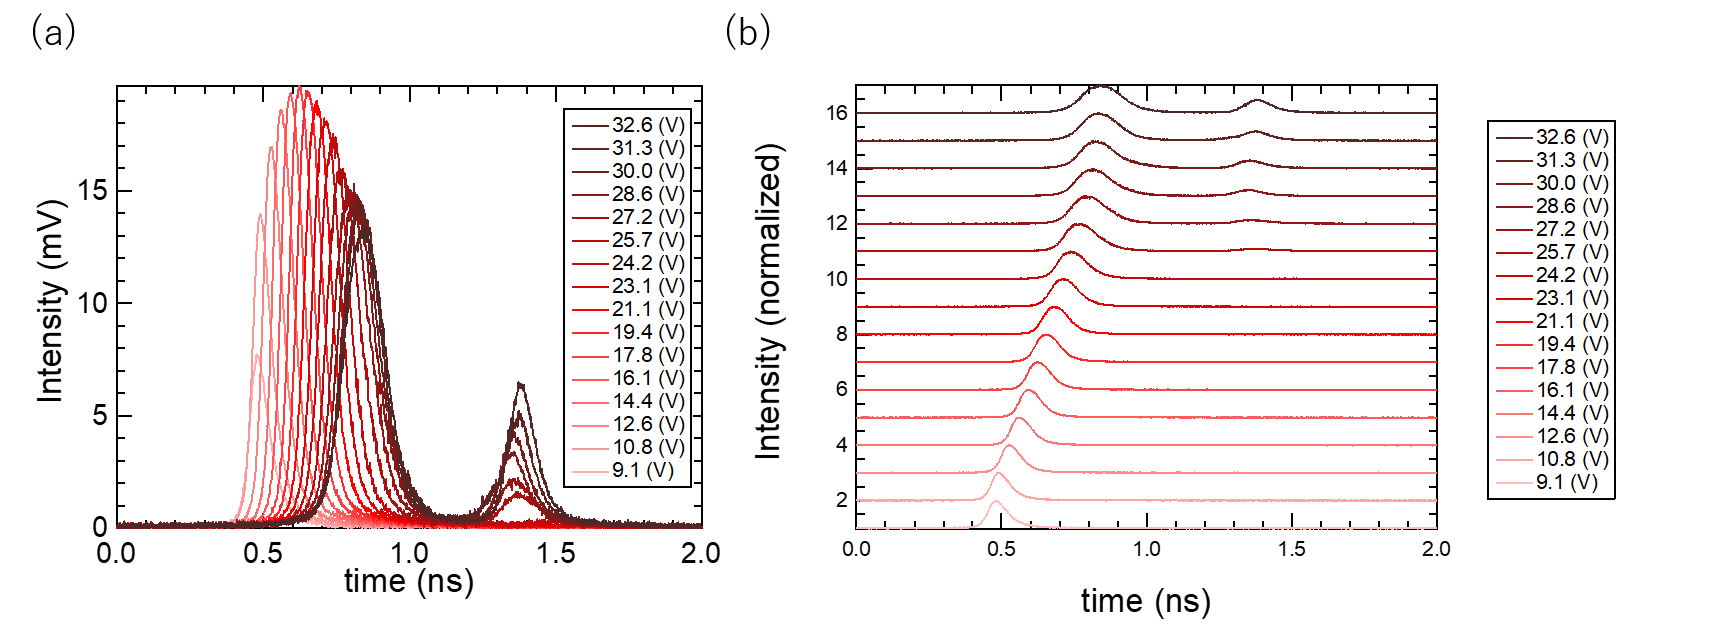
\includegraphics[width=15cm]{figure/fig_3_2_3QW_ridge_L200_GS.png}
		\caption{3周期歪量子井戸レーザー $L$=200 \si{\micro\metre} の利得スイッチング光パルスの時間波形}
		\label{fig:fig_3_2_3QW_ridge_L200_GS}
\end{figure}



図\ref{fig:fig_3_2_3QW_ridge_L300_GS}には$L$=300 \si{\micro\metre}試料の結果を示す。(a)の青い矢印は第1ピークの\adsp02{位置と強度}の移り変わりを表している。(a)を見ると第1パルスは一度極大値を持ったのち小さくなっている。また途中から第2パルスが見られるようになり第2パルスの方が第1パルスよりも大きくなる場合が見られる。(b)を見ると励起強度を上げていくと20.0 Vまではシングルパルスであることがわかる。20.0 Vで立ち上がり時間が遅くなり、それ以上の励起強度では複数のピークを持ったまま立ち上がり時間が早くなっていく様子がわかる。
%長い電流パルスの影響による緩和振動であると考えられる。
\begin{figure}[h]
	\centering
	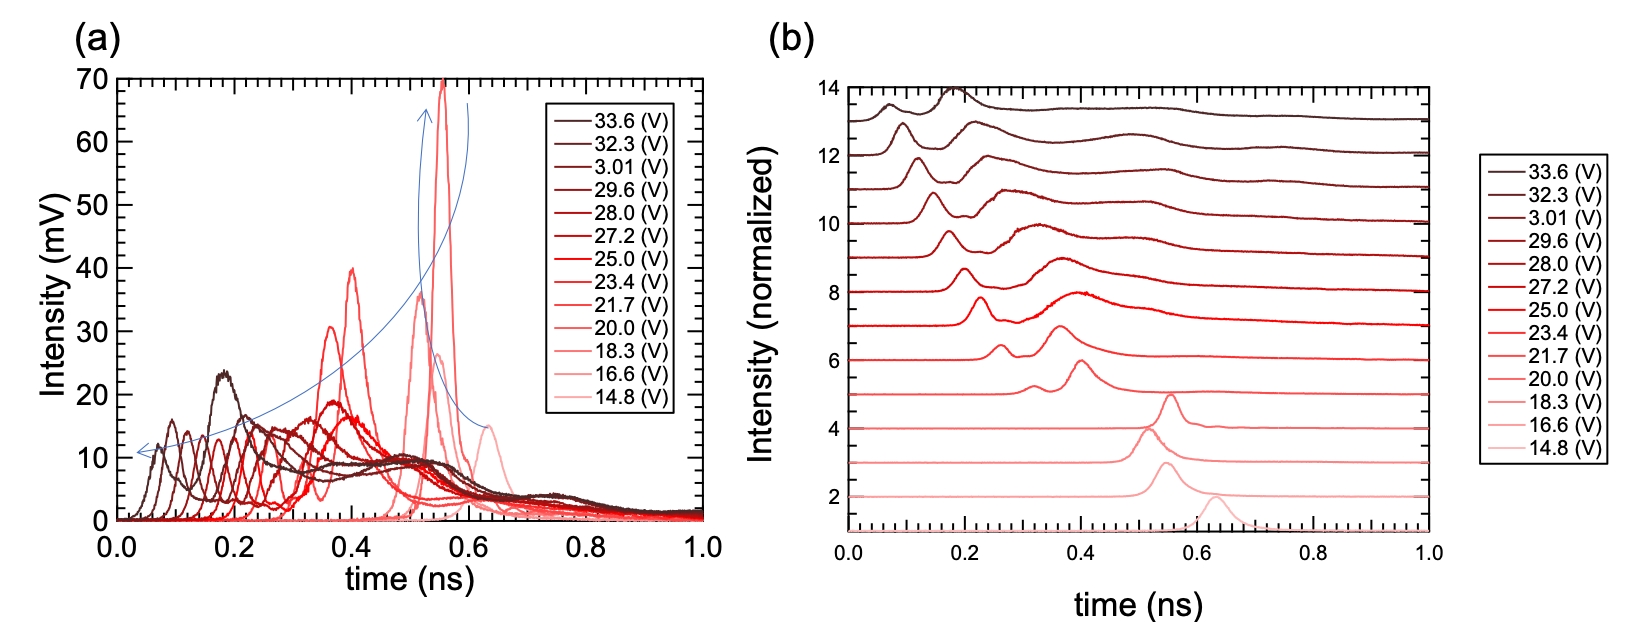
\includegraphics[width=15cm]{figure/fig_3_2_3QW_ridge_L300_GS.png}
		\caption{3周期歪量子井戸レーザー$ L$=300 \si{\micro\metre} の利得スイッチング光パルスの時間波形}
		\label{fig:fig_3_2_3QW_ridge_L300_GS}
\end{figure}


$L$=100 \si{\micro\metre}、200 \si{\micro\metre}、$L$=300 \si{\micro\metre}で見られた励起強度を大きくするに従って立ち上がりが遅くなる現象は通常の利得スイッチングの動作とは異なる。
%その原因は励起パルスが正常に印加されていないためではないかと考えられる。どの試料も配線する際の金線の長さが長く\delsp02{、インピーダンスが大きくなってしまったため、}短い電圧パルスが形を保てなかったと同時に励起強度も低くなってしまったと推測できる。
\subsubsection{3周期歪量子井戸リッジ導波路型レーザーの利得スイッチング動作実験のまとめ}
どの共振器試料においても典型的な利得スイッチングパルスの振る舞いは見られなかった。特にパルス形状が崩れてしまった原因は試料のマウントのためだと考えられる。


ここで利得スイッチング光パルスの第1パルスのパルス幅を示す。ここでパルス幅は半値全幅FWHMとしている。また光の検出に用いた25 GHzフォトダイオードによるパルス広がりを考慮してdeconvolutionを行った結果を示す。

図\ref{fig:fig_3_2_3QW_ridge_GS_FWHM}に3周期歪量子井戸リッジ導波路型レーザーの利得スイッチング光パルスのパルス幅を示す。縦軸FWHM、横軸が励起強度である。色分けは共振器長の違いを表す。

$L$=100 \si{\micro\metre}、200 \si{\micro\metre}では励起強度を上げるとパルス幅が長くなっている。\delsp02{これはインピーダンスマッチが取れていない事による電気パルスの変形だと考えられる。}$L$=300 \si{\micro\metre}ではパルス幅30 ps程度の値を示し一定値となった。最短パルス幅はL=300 \si{\micro m}、23.4 V印加で28.9 psであった。
\begin{figure}[ht]
	\centering
	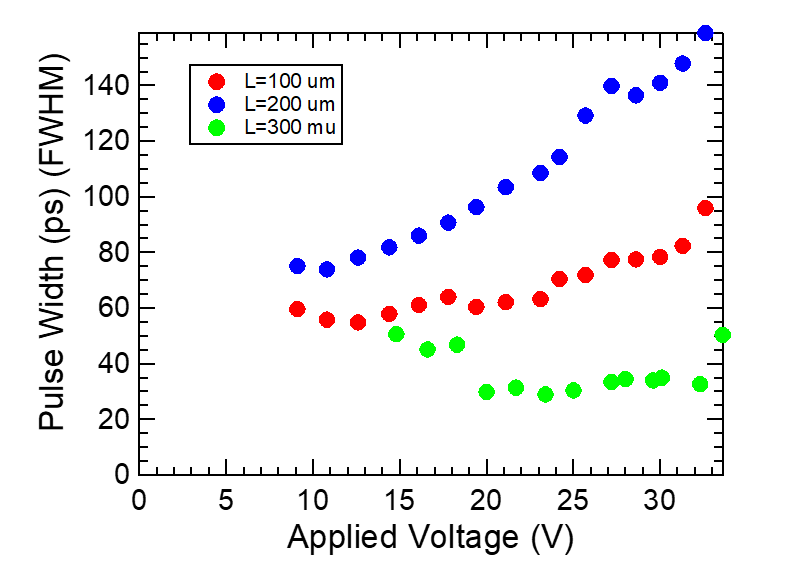
\includegraphics[width=10cm]{figure/fig_3_2_3QW_ridge_GS_FWHM.png}
		\caption{3周期歪量子井戸リッジ導波路型レーザーの光パルス幅}
		\label{fig:fig_3_2_3QW_ridge_GS_FWHM}
\end{figure}
\clearpage
\subsection{10周期歪補償量子井戸リッジ導波路型レーザーの利得スイッチング動作}%==============================
次に10周期歪補償量子井戸試料の利得スイッチング時間波形の結果を示す。

図\ref{fig:fig_3_2_10QW_ridge_L300_GS}には共振器長300 \si{\micro\metre}の結果を示す。(a)は時間波形の生データ、(b)は規格化したデータである。(a) を見ると励起強度をあげるにしたがって第1ピーク強度は大きくなっている。(b)を見ると最初はシングルピークだった光パルスが27 Vを超えたところから緩和振動とみられる複数のピークが観測された。第1ピークは励起強度とともに早く立ち上がる様子が見られる。典型的な利得スイッチング動作である。
\begin{figure}[h]
	\centering
	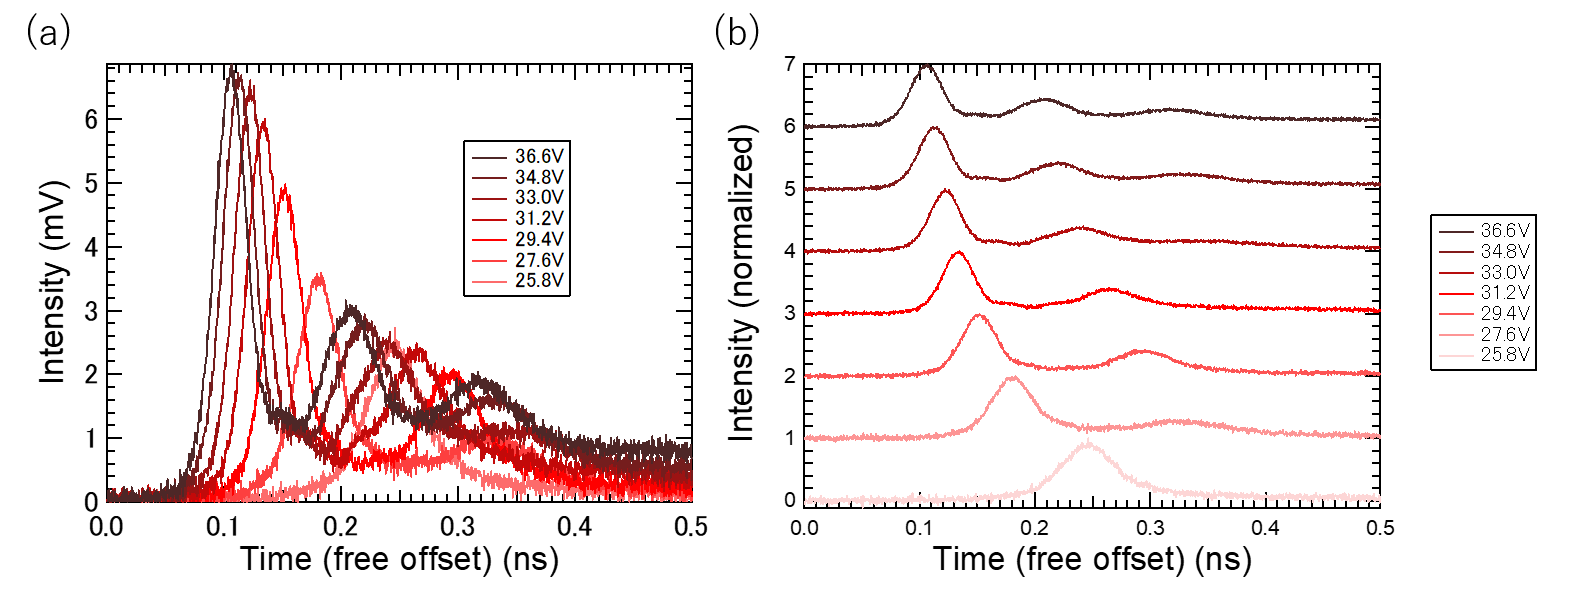
\includegraphics[width=15cm]{figure/fig_3_2_10QW_ridge_L300_GS.png}
		\caption{10周期歪補償量子井戸リッジ導波路型レーザー $L$=300 \si{\micro\metre} の利得スイッチング光パルスの時間波形}
		\label{fig:fig_3_2_10QW_ridge_L300_GS}
\end{figure}


図\ref{fig:fig_3_2_10QW_ridge_L400_GS}には共振器長$L$=400 \si{\micro\metre}の試料の結果を示す。(a)を見ると第1ピークは励起強度とともに大きくなっていく様子が見える。(b)を見ると励起強度を上げると緩和振動と見られる振動が見られるようになっていくことがわかる。また第1ピークの立ち上がり時間が早くなっている。
\begin{figure}[h]
	\centering
	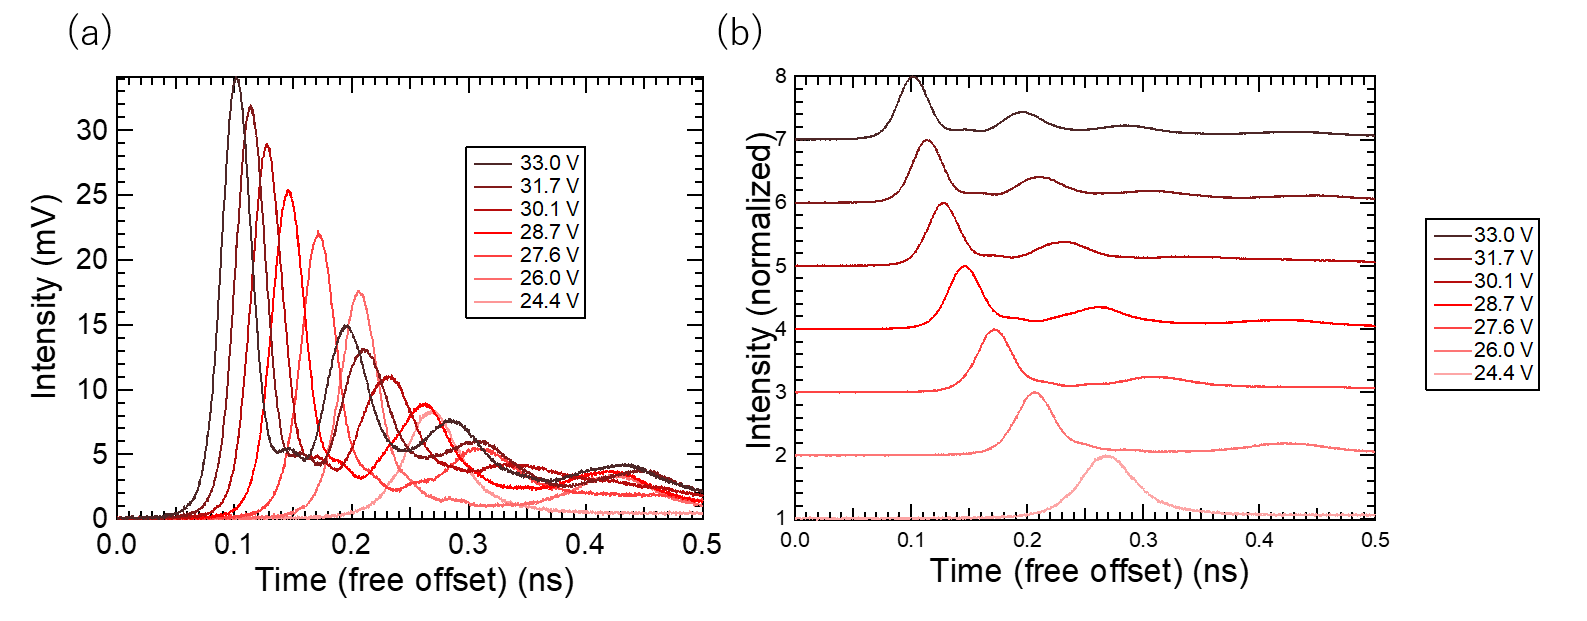
\includegraphics[width=15cm]{figure/fig_3_2_10QW_ridge_L400_GS.png}
		\caption{10歪補償量子井戸リッジ導波路型レーザー $L$=400 \si{\micro\metre} の利得スイッチング光パルスの時間波形}
		\label{fig:fig_3_2_10QW_ridge_L400_GS}
\end{figure}

%横軸の時間同じにできないの?
図\ref{fig:fig_3_2_10QW_ridge_L500_GS}に共振器長$L$=500 \si{\micro\metre}の試料の時間波形を示す。(a)を見ると第1ピークが励起強度とともに増大していくことがわかる。(b)を見ると励起強度の増大とともに立ち上がり時間が早くなっている。さらに26.6 Vを超えると緩和振動と見られるの第2パルスが見られ始める。
\begin{figure}[h]
	\centering
	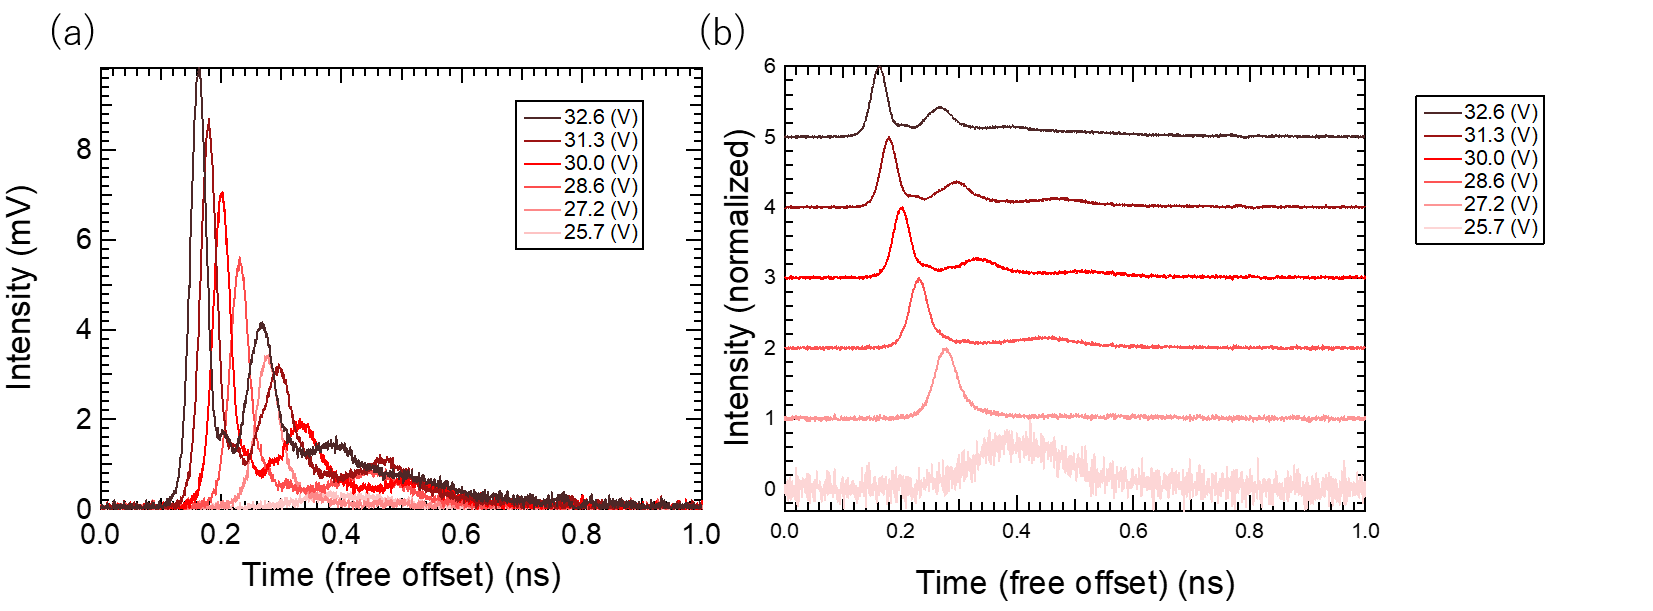
\includegraphics[width=15cm]{figure/fig_3_2_10QW_ridge_L500_GS.png}
		\caption{10周期歪補償量子井戸リッジ導波路型レーザー $L$=500 \si{\micro\metre} の利得スイッチング光パルスの時間波形}
		\label{fig:fig_3_2_10QW_ridge_L500_GS}
\end{figure}

\newpage
\subsubsection{10周期歪補償量子井戸リッジ導波路型レーザーの利得スイッチング動作実験のまとめ}
10周期歪補償量子井戸リッジ導波路型レーザーについてはどの全ての共振器長の試料についても典型的な利得スイッチング動作が見られた。


次図\ref{fig:fig_3_2_10QW_ridge_GS_FWHM}に10周期歪補償量子井戸リッジ導波路型レーザーの利得スイッチングパルスのパルス幅を示す。色分けは共振器長の違いを表す。
励起強度を増加していくとパルス幅は短くなる様子がどの共振器長でも見て取れる。$L$=300 \si{\micro\metre}では30 Vより強励起ではパルス幅は短くなることはなく29 ps程度で横ばいになっている。$L$=400 \si{\micro\metre}、$L$=500 \si{\micro\metre}でも印加電圧30 V付近でパルス幅の変化が小さくなっており、飽和が起きている。最短パルス幅は$L$=400 \si{\micro\metre}で26.5 psであった。共振器長依存性は見られなかった。
\begin{figure}[h]
	\centering
	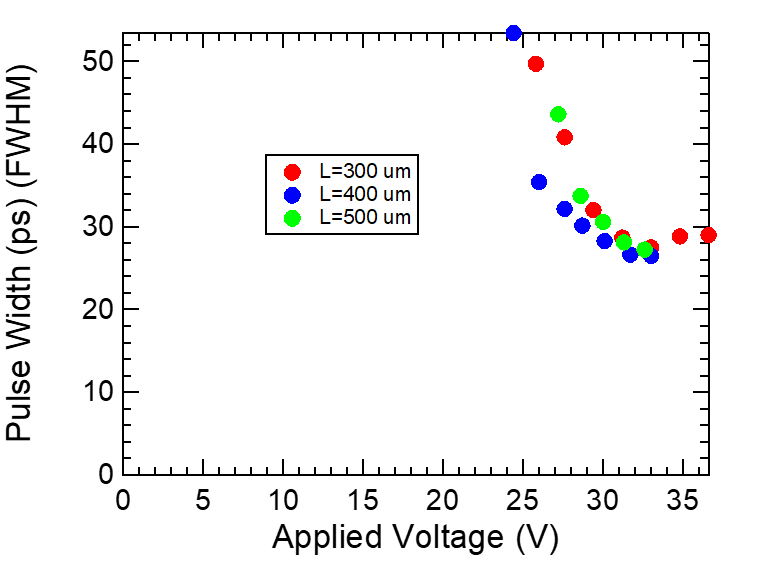
\includegraphics[width=10cm]{figure/fig_3_2_10QW_ridge_GS_FWHM.png}
		\caption{10周期歪補償量子井戸リッジ導波路型レーザーの光パルス幅}
		\label{fig:fig_3_2_10QW_ridge_GS_FWHM}
\end{figure}

\subsection{利得スイッチング動作実験のまとめ}%===========================

3周期歪量子井戸リッジ導波路型レーザーと10周期歪補償量子井戸リッジ導波路型レーザーについての利得スイッチング実験の結果をまとめる。


\subsubsection{3周期歪量子井戸レーザーと10周期歪補償レーザーの結果の比較}
3周期歪量子井戸レーザーにおいて、$L$=100 \si{\micro\metre}と200 \si{\micro\metre}については試料のマウントの方法に問題があり典型的な利得スイッチングパルスは得られなかった。共振器長が$L$=300 \si{\micro\metre}試料では最短パルス幅23.4 V印加で28.9 psであった。

10周期歪補償量子井戸レーザーについては典型的な利得スイッチングパルスが得られ、最短パルス幅は$L$=400 \si{\micro\metre}で26.5 psであった。

3周期試料と10周期試料ではどちらも30 ps程度に収束しておりモード利得の違いによるパルス幅の差異が明確ではないと考えられる。

%パルス幅を制限する外的要因として駆動電気パルスの立ち上がり時間について詳細に調べることで解明が可能であると考えられる。
\subsubsection{測定されたパルス幅の要因に関する考察}
先行研究によると理想的には利得スイッチングパルスの立ち上がりの限界のはやさはモード利得、立ち下がりの限界のはやさは共振器寿命によって決定された。
そこで式(\ref{eq:tau_p})を用いて共振器寿命を計算してみると表\ref{table:table_taup}のようになる。
\begin{table}[h]
  \caption{共振器寿命}
  \label{table:table_taup}
  \centering
  \begin{tabular}{lccc}
    \hline
    試料   &  内部損失$\alpha_{int} \rm{ /cm}$&共振器長  \si{\micro\metre} &共振器寿命 $\tau_{p}$  ps \\
    \hline \hline
     3周期歪量子井戸 &   11.8 &300 &2.3\\
    10周期歪補償量子井戸  & 18.0 &300&2.01\\
    \hline
  \end{tabular}
\end{table}

計算にはR=0.3, $n_{eq}$=3.5を用いた。

実験結果はパルス幅数十psであるので共振器寿命よりも1桁大きくなっている。共振器寿命のパルス幅の決定への寄与は小さいと考えれ、共振器長を変えたときにパルス幅が変わらなかったのはそのためだと考えられる。

またモード利得から算出される立ち上がり時間の計算を行った。立ち上がり時間$\tau_{rise}$は
\begin{eqnarray}
\tau _{rise}=\nu _{g}\left\lbrace  \Gamma g - \dfrac{1}{\nu_{g}\tau_{p}}\right\rbrace 
\end{eqnarray}
で与えられ、$\nu_{g}=7.3\times10^{-3} \ \si{cm/ps}$\cite{ref_takashi_ito}、 $\tau_{p}=2.0 \ \si{ps}$、 $\Gamma g=100\ \si{/cm}$とすると$\tau_{rise}=4.4\ \si{ps}$と計算される。立ち上がり時間も共振器寿命と同様に測定結果のパルス幅30 ps程度よりも十分短い。測定で得られたパルス幅はモード利得や共振器寿命とは別の要因によって律則されていることが示唆される。


パルス幅を決める要因として励起強度に注目し、励起密度を変えてレート方程式に基づく光子密度とキャリア密度の時間発展の数値計算を行った。図\ref{fig:fig_3_2_GS_sim}に利得スイッチングパルスの励起強度依存性の数値計算結果を示す。インパルス励起を考えた。励起強度を大きくしていくに従ってパルス幅が短くなり、立ち上がりも早くなる振る舞いがわかる。また理想的に高密度励起した場合にはモード利得や共振器寿命程度の時間スケールのパルス幅が得られるのに対し、弱励起においては非常に長いパルス幅が発生することがわかる。本研究で得られたパルス幅も励起強度十分でなかったためにパルス幅が共振器寿命の時間スケールよりも長くなったと考えられる。

%求めるパルス幅を得るためには
十分な励起強度をまた十分短い時間のうちに
%(電気パルスの立ち上がり)
注入することで上で計算し立ち上がり時間や立ち下がり時間の効果が見えるようなパルス幅が得られる。本研究におけるナノ秒電流注入測定においては電気回路の高速性が不十分であったため、それが達成されなかったと考えられる。
\begin{figure}[h]
	\centering
	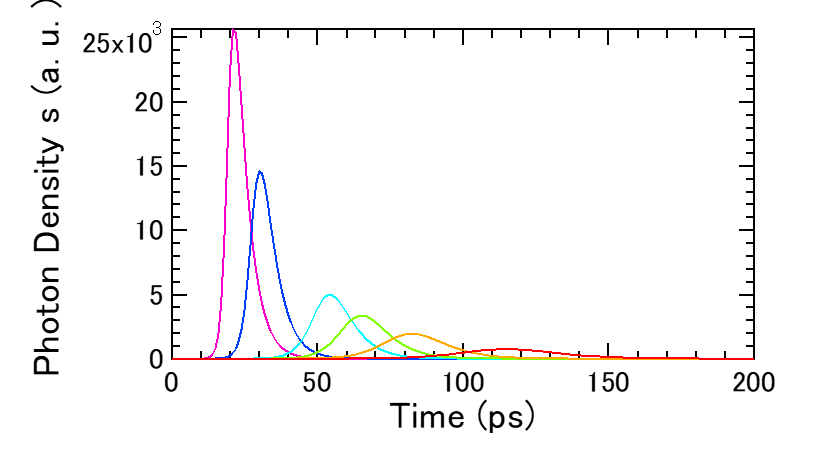
\includegraphics[width=15cm]{figure/fig_3_2_GS_sim.png}
		\caption{利得スイッチングパルスの励起強度依存性の数値計算結果}
		\label{fig:fig_3_2_GS_sim}
\end{figure}

